\documentclass[11pt]{article}

% -------------------------------------------------
% Packages
% -------------------------------------------------
\usepackage[T1]{fontenc}
\usepackage[utf8]{inputenc}
\usepackage{lmodern}

\usepackage[margin=1in]{geometry}
\usepackage{setspace}
\doublespacing

\usepackage{amsmath,amssymb,amsthm,mathtools}
\usepackage{bm}
\usepackage{booktabs}
\usepackage{graphicx}
\usepackage{tikz}
\usepackage{pgfplots}
\pgfplotsset{compat=1.18}
\usepackage{enumitem}
\usepackage{xcolor}
\usepackage{xurl}
\usepackage{hyperref}
\usepackage[round,authoryear]{natbib}

\hypersetup{
  colorlinks=true,
  linkcolor=blue,
  citecolor=blue,
  urlcolor=blue,
  pdftitle={Entry Subsidies under Buyout Exit: Merger Policy, Project Orientation, and the Local--National Incidence Wedge},
  pdfauthor={Ryota Matsuki},
  pdfkeywords={startup subsidies, acquisitions, merger policy, project orientation, entrepreneurship, incidence-based policy}
}

% -------------------------------------------------
% Theorem environments
% -------------------------------------------------
\theoremstyle{plain}
\newtheorem{assumption}{Assumption}
\newtheorem{proposition}{Proposition}
\newtheorem{corollary}{Corollary}
\newtheorem{lemma}{Lemma}

\theoremstyle{remark}
\newtheorem{remark}{Remark}

% -------------------------------------------------
% Title
% -------------------------------------------------
\title{Entry Subsidies under Buyout Exit:\\
Merger Policy, Project Orientation, and the Local--National Incidence Wedge}

\author{Ryota Matsuki\thanks{Corresponding author. Email: \texttt{ryota.matsuki@gmail.com}. This work was conducted in a personal capacity; the views expressed are solely those of the author.}\\
\small Independent Researcher, Matsuyama, Ehime, Japan\\
\small Corresponding author: \texttt{ryota.matsuki@gmail.com}}

\date{}

% -------------------------------------------------
% Document
% -------------------------------------------------
\begin{document}

\maketitle

\begin{abstract}
This paper studies startup subsidies when entrepreneurial success often leads to acquisition rather than independent competition. Entrepreneurs choose whether to enter, how much effort to exert, and whether to pursue an independence-oriented or buyout-oriented project. Throughout, the approval parameter is a reduced-form summary of merger permissiveness or, more broadly, exit realizability. A more permissive exit environment raises entry and effort by improving exit options, but it can also redirect entrepreneurial project choice toward buyout-oriented projects. Because a uniform entry subsidy does not affect project choice, it cannot correct that composition distortion. Consequently, easier buyout exit can reduce the optimal subsidy and alter the relevant local--national incidence wedge.
\end{abstract}

\noindent
\textbf{Keywords:} startup subsidies; acquisitions; merger policy; project orientation; entrepreneurship; incidence-based policy

\noindent
\textbf{JEL codes:} L13; L26; L41; O31

\newpage

\section{Introduction}\label{sec:intro}

Governments devote substantial resources to startup promotion, especially at the local level, where such policies are justified by expected gains in innovation, competition, and regional spillovers. Yet many successful startups do not remain independent competitors. Instead, they exit through acquisition by incumbents. This raises a basic question: when buyout exit is pervasive, does subsidizing startup entry create socially valuable competition, or does it instead expand the supply of firms built to sell out?

This paper studies entry subsidies in an environment in which prospective entrepreneurs choose whether to enter, how much effort to exert, and whether to pursue an independence-oriented or a buyout-oriented project. The former is stronger as a stand-alone business; the latter is more valuable under acquisition. After success, the entrant and the incumbent may attempt a merger, which is approved with probability \(q\). A government chooses an entry subsidy before entry takes place. In the baseline, \(q\) should be read as a reduced-form summary of exit realizability: merger policy is one interpretation, but not the only one. Throughout, entrepreneurial direction refers to the direction of project choice between stand-alone-oriented and buyout-oriented entrepreneurship.

The core mechanism is straightforward. A more permissive merger environment raises the private value of entrepreneurship by improving the entrepreneur's exit option, but it also changes the direction of entrepreneurial project choice. When acquisition becomes sufficiently attractive, entrepreneurs shift from independence-oriented projects toward buyout-oriented projects. Because a uniform entry subsidy does not affect project choice, it cannot correct that composition margin; it only scales entry at the privately preferred project margin. As a result, easier buyout exit need not strengthen the case for startup subsidies and can instead reduce the optimal subsidy.

A second key point is methodological. A merger is not always attempted after startup success; it is attempted only when expected merger gains cover filing and implementation costs. Welfare analysis must therefore respect the same behavioral margins that govern private equilibrium. Once this is imposed, merger policy affects subsidy design only when it changes actual behavior.

The paper makes three contributions. First, unlike the literature on acquisitions and merger policy \citep{cunningham2021killer,letina2024killer,dijk2024direction,dijk2025strategic}, which studies how acquisition prospects affect innovation strategy and competition, this paper studies subsidy design when buyout exit jointly shapes entry, effort, and project orientation. The analytical novelty is a behaviorally consistent welfare framework: merger attempt is endogenous, so the same attempt margin must enter both private continuation values and welfare accounting. Section \ref{sec:subsidy} therefore derives a primitive benchmark in which the main subsidy formulas and comparative statics are pinned down by product-market primitives together with the merger-attempt condition alone. Second, unlike the literature on entrepreneurial finance and public startup support \citep{lerner2020vcrole,lerner2022governmentincentives,bai2021public}, which typically asks whether public support increases startup formation or financing, this paper shows that stronger exit opportunities can raise private incentives while weakening the social case for subsidy by redirecting entrepreneurship toward buyout-oriented projects. Uniform entry subsidies therefore scale entry but do not correct project composition. Third, unlike place-based policy work that emphasizes strategic competition across jurisdictions or generic local spillovers, this paper derives a local--national \emph{incidence} wedge around that primitive benchmark. For a fixed project, the wedge reflects planner-specific incidence weights; what buyout exit adds is that merger permissiveness can change which project is privately selected, thereby changing the economically relevant local--national comparison. Appendices \ref{app:sufficientlocalover} and \ref{app:sufficientlocalunder} develop the economic content of that incidence comparison. The clawback exercise in Section \ref{sec:extensions} illustrates instrument separation rather than constituting the paper's main analytical contribution.

These results matter for a broad set of startup policies, including grants, tax credits, accelerators, multilevel startup support, and broader startup policy packages \citep{fazio2020rdtax,denes2023investortax,gonzalezuribe2018accelerators,manaresi2021startupact,lanahan2015multilevel}. The main implication is that policy should not ask only whether support increases startup formation. It must also ask what kinds of startups are being created and whether public support reinforces incentives to build independent competitors or acquisition targets. Section \ref{sec:extensions} returns to this point through an illustrative clawback exercise that shows how an additional instrument can target the composition margin without changing the paper's core welfare logic.

The remainder of the paper is organized as follows. Section \ref{sec:related} reviews the related literature. Section \ref{sec:model} presents the model. Section \ref{sec:private} characterizes private equilibrium project choice, effort, and entry. Section \ref{sec:subsidy} derives the primitive benchmark subsidy under buyout exit. Section \ref{sec:decentralized} adds local and national incidence extensions around that benchmark. Section \ref{sec:extensions} considers extensions and policy design. Section \ref{sec:conclusion} concludes.

\section{Related Literature}\label{sec:related}

This paper relates to three strands of literature: acquisitions and innovation, entrepreneurial finance and startup policy, and local versus national policy evaluation.

The closest connection is to the literature on acquisitions of innovative entrants and their effects on innovation and competition. \citet{cunningham2021killer} show that acquisitions can eliminate future competition by shutting down overlapping innovation projects. Subsequent theoretical work has broadened that perspective. \citet{letina2024killer} study how merger policy affects innovation strategies more generally, while \citet{dijk2024direction} and \citet{dijk2025strategic} analyze how acquisition prospects distort startup innovation and R\&D incentives. Our paper builds on these insights but asks a different question: how should entry subsidies be designed when buyout exit and merger review jointly shape project choice and the social value of successful entry?

The paper also connects to the literature on value capture in startup markets. \citet{arora2024missing} emphasize that startups often rely on external buyers or downstream partners to realize returns. That perspective is central here: buyout exit is not a secondary outcome but a determinant of private entrepreneurial incentives before the product market is reached.

A second related literature studies entrepreneurial finance and public startup support. \citet{lerner2020vcrole}, \citet{lerner2022governmentincentives}, and \citet{bai2021public} discuss venture capital, public entrepreneurial finance, and government support for startups. Empirical work evaluates instruments such as R\&D tax credits, investor tax credits, accelerators, multilevel startup support, and broader startup policy packages \citep{fazio2020rdtax,denes2023investortax,gonzalezuribe2018accelerators,lanahan2015multilevel,manaresi2021startupact}. Our paper is complementary to that literature: rather than estimating treatment effects, it develops a theory of why the effectiveness of startup subsidies depends on the acquisition environment and why stronger private entry incentives need not imply stronger grounds for subsidy.

The third relevant literature concerns geography and the divergence between local and national policy evaluation. \citet{chen2010buylocal} and \citet{chatterji2014clusters} motivate attention to local entrepreneurial ecosystems. \citet{kline2013peopleplaces} provide a foundational framework for understanding why local and national welfare effects of place-based policy can differ. Our mechanism is different. We do not model strategic subsidy competition across jurisdictions. Instead, we study how buyout exit changes the incidence of gains and losses from startup policy, thereby generating a local--national incidence wedge even when the underlying private equilibrium is the same.

Relative to these literatures, the paper's novelty is not simply to add acquisitions to a startup-subsidy model. It combines three elements that are usually studied separately. First, it embeds endogenous merger attempt into both private incentives and welfare accounting, yielding a primitive benchmark subsidy formula driven by product-market primitives and the merger-attempt condition. Second, it makes entrepreneurial direction a choice variable, so merger permissiveness changes not only how much entrepreneurship occurs but also what type occurs; a uniform subsidy cannot correct that composition distortion. Third, it shows that the local--national wedge is not only an incidence comparison for a fixed project: because buyout exit can trigger project switching, the economically relevant wedge can itself change with the exit environment.

\section{Model}\label{sec:model}

This section develops a tractable model of startup subsidies, buyout exit, and merger review.
The key ingredients are a local entry subsidy, a post-entry choice between an independence-oriented and a buyout-oriented project, and a reduced-form merger approval probability that governs the attractiveness of acquisition as an exit route.

\subsection{Environment and timing}

Consider a unit measure of independent local markets indexed by \(m \in [0,1]\).
In each market there is one incumbent firm and one potential startup project.
Markets are otherwise identical, except that potential entrants differ in their fixed entry costs.
A local government offers a uniform entry subsidy \(s \ge 0\) to any entrepreneur who enters.

In each market, the timing is as follows:

\begin{enumerate}
    \item The local government chooses a uniform entry subsidy \(s\).
    \item The potential entrepreneur in market \(m\) observes an idiosyncratic fixed cost \(f_m\) and decides whether to enter.
    \item Conditional on entry, the entrepreneur chooses a project type \(j \in \{I,B\}\) and an effort level \(x \in [0,1]\).
    \item If the project succeeds, the incumbent and the entrant bargain over a potential merger.
    \item If a merger is attempted, it is approved with probability \(q \in [0,1]\).
    \item If the merger is approved, the merged firm operates in the product market; otherwise the incumbent and the entrant compete as independent firms.
\end{enumerate}

We interpret \(q\) as a reduced-form measure of merger permissiveness.
A higher \(q\) corresponds to a more permissive merger environment, or more generally to an environment in which buyout exit is easier to realize.
The baseline keeps this shift project-invariant in order to focus on project choice and welfare accounting in a one-dimensional way; Appendix \ref{app:typespecificq} briefly notes how the mechanism extends when approval or exit realizability differs across project types.
To avoid confusion, \(q\) is the approval or exit-realizability parameter, whereas \(q_I\) and \(q_E\) below denote product-market quantities.

The entry cost \(f_m\) is independently drawn from the uniform distribution on \([0,1]\).
The uniform specification is used for closed-form results in the main text; the appendices show how the analysis extends to a general distribution \(G(f)\).

\subsection{Product-market payoffs}

If entry succeeds, the product-market primitives depend on the entrepreneur's project choice \(j \in \{I,B\}\).
Type \(I\) denotes an \emph{independence-oriented} project: it is relatively strong as a stand-alone business.
Type \(B\) denotes a \emph{buyout-oriented} project: it is relatively attractive as an acquisition target.
These two project types should be read as reduced-form project orientations rather than as a fully dynamic innovation-race model.
The primitive differences \((a_j,\sigma_j,m_j)\) capture, respectively, stand-alone marketability, product overlap with the incumbent, and acquisition-specific integration value or rents.

For a successful entrant of type \(j\), inverse demands are given by
\begin{align}
    p_I &= 1 - q_I - \sigma_j q_E, \\
    p_E &= a_j - q_E - \sigma_j q_I,
\end{align}
where \(q_I\) and \(q_E\) denote the incumbent's and entrant's quantities, respectively,
\(a_j > 0\) is the entrant's stand-alone demand shifter, and \(\sigma_j \in (0,1)\) captures substitutability between the incumbent's and the entrant's products.
Marginal costs are normalized to zero.

We impose parameter restrictions ensuring interior product-market solutions under both independent competition and common ownership:
\begin{equation}\label{eq:interiorpm}
    \sigma_j < a_j < \frac{1}{\sigma_j},
    \qquad j \in \{I,B\}.
\end{equation}

\paragraph{Independent competition.}
If no merger takes place, the incumbent and the entrant compete \`a la Cournot.
The incumbent solves
\begin{equation}
    \max_{q_I \ge 0}\; (1-q_I-\sigma_j q_E)q_I,
\end{equation}
and the entrant solves
\begin{equation}
    \max_{q_E \ge 0}\; (a_j-q_E-\sigma_j q_I)q_E.
\end{equation}
The unique interior Nash equilibrium is
\begin{align}
    q_I^D(j) &= \frac{2-a_j\sigma_j}{4-\sigma_j^2}, \\
    q_E^D(j) &= \frac{2a_j-\sigma_j}{4-\sigma_j^2}.
\end{align}
At this equilibrium, prices satisfy
\begin{equation}
    p_I^D(j)=q_I^D(j),
    \qquad
    p_E^D(j)=q_E^D(j),
\end{equation}
so profits are
\begin{align}
    \pi_I^D(j) &= \left(\frac{2-a_j\sigma_j}{4-\sigma_j^2}\right)^2, \\
    \pi_E^D(j) &= \left(\frac{2a_j-\sigma_j}{4-\sigma_j^2}\right)^2.
\end{align}

Consumer surplus under independent ownership is
\begin{equation}\label{eq:csd}
    C^D(j)
    =
    \frac{1}{2}
    \left[
        \bigl(q_I^D(j)\bigr)^2
        + \bigl(q_E^D(j)\bigr)^2
        + 2\sigma_j q_I^D(j)q_E^D(j)
    \right].
\end{equation}

\paragraph{Approved merger.}
If the entrant is acquired and the merger is approved, the merged firm chooses \((q_I,q_E)\) to maximize joint operating profit.
In addition, common ownership generates a type-specific synergy \(m_j \ge 0\), which captures the private value of integrating the entrant's technology, customer base, team, or complementary assets into the incumbent.

The merged firm solves
\begin{equation}
    \max_{q_I,q_E \ge 0}\;
    (1-q_I-\sigma_j q_E)q_I
    +
    (a_j-q_E-\sigma_j q_I)q_E
    +
    m_j.
\end{equation}
The unique interior solution is
\begin{align}
    q_I^M(j) &= \frac{1-a_j\sigma_j}{2(1-\sigma_j^2)}, \\
    q_E^M(j) &= \frac{a_j-\sigma_j}{2(1-\sigma_j^2)}.
\end{align}
The corresponding operating profit is
\begin{equation}
    \Pi_{\mathrm{op}}^M(j)
    =
    \frac{a_j^2 - 2a_j\sigma_j + 1}{4(1-\sigma_j^2)},
\end{equation}
so total merged profit is
\begin{equation}
    \Pi^M(j) = \Pi_{\mathrm{op}}^M(j) + m_j.
\end{equation}
Consumer surplus under common ownership is
\begin{equation}\label{eq:csm}
    C^M(j)
    =
    \frac{1}{2}
    \left[
        \bigl(q_I^M(j)\bigr)^2
        + \bigl(q_E^M(j)\bigr)^2
        + 2\sigma_j q_I^M(j)q_E^M(j)
    \right].
\end{equation}

Define the private merger surplus for project \(j\) as
\begin{equation}\label{eq:Deltaj}
    \Delta_j \equiv \Pi^M(j) - \pi_I^D(j) - \pi_E^D(j).
\end{equation}

The two project types differ in their stand-alone and acquisition properties.
Throughout, we assume that type \(I\) is more attractive under independent ownership, whereas type \(B\) generates a larger private gain from acquisition.

\begin{assumption}\label{ass:types}
The product-market primitives satisfy
\begin{equation}
    \pi_E^D(I) > \pi_E^D(B)
    \qquad \text{and} \qquad
    \Delta_B > \Delta_I > 0.
\end{equation}
\end{assumption}

Assumption \ref{ass:types} captures the intended distinction between the two project types.
A sufficient primitive configuration is that type \(I\) has a higher stand-alone demand shifter, whereas type \(B\) features a larger synergy term \(m_j\) and/or higher substitutability \(\sigma_j\), making it more valuable under common ownership.
In that sense, the model's notion of entrepreneurial direction is the direction of project orientation between stand-alone competition and buyout exit.

\subsection{Project choice, effort, and entry}

After entering, the entrepreneur chooses a project type \(j \in \{I,B\}\) and an effort level \(x \in [0,1]\).
Effort is interpreted as the probability of technical and commercial success.
Its cost is
\begin{equation}
    c(x) = \frac{x^2}{2}.
\end{equation}

If the project succeeds, the entrepreneur obtains a project-specific continuation payoff that depends on whether a merger is attempted and approved.
Let \(R_j(q)\) denote the entrepreneur's expected continuation payoff conditional on success and project choice \(j\).
Given \(R_j(q)\), the entrepreneur solves
\begin{equation}
    \max_{x \in [0,1]} \; xR_j(q) - \frac{x^2}{2}.
\end{equation}

Hence, before success is realized, the entrepreneur's expected payoff from entering with project \(j\) and fixed cost \(f_m\) is
\begin{equation}
    U_j(f_m;s,q)
    =
    s - f_m
    + \max_{x \in [0,1]}
      \left\{
        xR_j(q) - \frac{x^2}{2}
      \right\}.
\end{equation}

The entrepreneur chooses the project type that maximizes \(U_j(f_m;s,q)\), and then decides whether to enter.
Thus entry occurs if and only if
\begin{equation}
    \max_{j \in \{I,B\}} U_j(f_m;s,q) \ge 0.
\end{equation}

We restrict attention to parameter values such that the optimal effort choice is interior in the main text.
Under this restriction, the entrepreneur's effort and entry decisions admit closed-form solutions characterized in the next section.

\subsection{Acquisition bargaining and merger review}

If a type-\(j\) project succeeds, the incumbent and the entrant may attempt a merger.
Filing and implementing the transaction requires a fixed cost \(k>0\), interpreted as the legal, administrative, and organizational cost of merger review and consummation.

The sequence is as follows.
After success is realized, the incumbent and the entrant observe project type \(j\) and bargain over the merger.
If they attempt a merger, approval occurs with probability \(q\); if approval is denied, the firms remain independent and compete in the product market.

We assume Nash bargaining over the \emph{expected} merger surplus, with the entrepreneur receiving bargaining weight \(\beta \in (0,1)\).
The no-merger outside options are \(\pi_I^D(j)\) and \(\pi_E^D(j)\).
If the firms attempt a merger, the expected joint payoff net of filing cost is
\begin{equation}
    q\Pi^M(j) + (1-q)\bigl(\pi_I^D(j)+\pi_E^D(j)\bigr) - k,
\end{equation}
whereas the outside option from not filing is
\begin{equation}
    \pi_I^D(j)+\pi_E^D(j).
\end{equation}
Hence the incremental expected gain from attempting the merger is
\begin{equation}
    q\Delta_j - k.
\end{equation}

The firms attempt a merger if and only if
\begin{equation}\label{eq:attemptcondition}
    q\Delta_j \ge k.
\end{equation}
Under Nash bargaining, the entrepreneur's expected continuation payoff conditional on success is therefore
\begin{equation}\label{eq:Rj}
    R_j(q)
    =
    \pi_E^D(j)
    +
    \beta \bigl[q\Delta_j-k\bigr]_+,
\end{equation}
where \([z]_+ \equiv \max\{z,0\}\).

Equation \eqref{eq:Rj} is central.
A higher approval probability \(q\) raises the attractiveness of project types with large merger surplus.
As a result, merger policy affects not only the quantity of entry, but also the direction of entrepreneurial innovation.

\subsection{Policy-relevant welfare ingredients}

The baseline policy instrument is the local entry subsidy \(s\). The government takes the merger approval probability \(q\) as given and chooses \(s\) before entry takes place.

For policy analysis, social value is built from consumer surplus, profit components, and non-pecuniary spillovers under either independent ownership or approved acquisition. Section \ref{sec:subsidy} first aggregates these primitives into a benchmark social value that depends only on product-market primitives and merger-attempt behavior. Section \ref{sec:decentralized} then adds local and national incidence weights on top of that benchmark. The crucial point is that merger attempt is endogenous: the same condition \eqref{eq:attemptcondition} that governs private continuation values must also govern welfare accounting. If \(q\Delta_j<k\), no merger is attempted and successful entry yields the independent-ownership value. If \(q\Delta_j \ge k\), a merger is attempted, approval occurs with probability \(q\), and the resource cost of attempt is incurred regardless of approval.

The next sections use this behaviorally consistent accounting to derive the primitive benchmark subsidy, then compare planner-specific local and national incidence extensions around that benchmark.

\section{Private Equilibrium}\label{sec:private}

This section characterizes the entrepreneur's private choices given the subsidy \(s\) and the merger approval probability \(q\).
We proceed in three steps.
First, we solve the entrepreneur's effort choice for each project type.
Second, we characterize private project choice as a function of merger permissiveness.
Third, we derive the entry cutoff and the resulting mass of entrants.

\subsection{Continuation values and effort}

Recall from \eqref{eq:Rj} that, conditional on success, the entrepreneur's continuation payoff under project \(j \in \{I,B\}\) is
\begin{equation}
    R_j(q)
    =
    \pi_E^D(j)
    +
    \beta \bigl[q\Delta_j-k\bigr]_+.
\end{equation}
Because \(\pi_E^D(j)>0\), each \(R_j(q)\) is strictly positive.
Moreover, by Assumption \ref{ass:types}, project \(I\) yields a larger stand-alone payoff,
whereas project \(B\) yields a larger gain from acquisition.

Let
\begin{equation}
    \bar q_j \equiv \frac{k}{\Delta_j},
    \qquad j \in \{I,B\},
\end{equation}
Because Assumption \ref{ass:types} implies \(\Delta_B>\Delta_I>0\), both merger-feasibility thresholds are well-defined, and
\begin{equation}
    \bar q_B < \bar q_I.
\end{equation}
Thus, as merger policy becomes more permissive, the buyout-oriented project becomes merger-feasible strictly before the independence-oriented project does.

The entrepreneur chooses effort \(x \in [0,1]\) to solve
\begin{equation}
    \max_{x \in [0,1]} \;
    xR_j(q)-\frac{x^2}{2}.
\end{equation}
The next assumption ensures that the main-text solution is interior.

\begin{assumption}\label{ass:interior}
For each \(j \in \{I,B\}\) and all \(q \in [0,1]\), the success-contingent return satisfies
\begin{equation}
    0 < R_j(q) < 1.
\end{equation}
In addition, for the equilibrium values of \(s\) and \(q\) considered in the main text,
\begin{equation}
    0
    <
    s + \frac{1}{2}\max\{R_I(q)^2,R_B(q)^2\}
    <
    1.
\end{equation}
\end{assumption}

Under Assumption \ref{ass:interior}, the entrepreneur's optimal effort under project \(j\) is
\begin{equation}\label{eq:xjstar}
    x_j^*(q)=R_j(q),
\end{equation}
and the corresponding ex ante private payoff from entering with project \(j\) is
\begin{equation}\label{eq:Uj}
    U_j(f;s,q)
    =
    s-f+\frac{R_j(q)^2}{2}.
\end{equation}

Since the subsidy \(s\) enters additively in \eqref{eq:Uj}, it affects the entry decision but does not affect the ranking of projects conditional on entry.
Accordingly, project choice is governed entirely by the comparison between \(R_I(q)\) and \(R_B(q)\).

\subsection{Project choice}

To obtain a clean threshold characterization in the main text, we impose a single-crossing condition.

\begin{assumption}\label{ass:singlecross}
The approval probability
\begin{equation}\label{eq:qhat}
    \hat q
    \equiv
    \frac{\pi_E^D(I)-\pi_E^D(B)}
         {\beta(\Delta_B-\Delta_I)}
\end{equation}
satisfies
\begin{equation}
    \hat q \in [\bar q_I,1).
\end{equation}
\end{assumption}

Assumption \ref{ass:singlecross} ensures that any switch toward the buyout-oriented project occurs only once both project types are merger-feasible.
Appendix \ref{app:projchoice} shows that without this restriction, private project choice is characterized by a simple piecewise threshold system.
The same economic mechanism survives in that more general case: project \(I\) is preferred for sufficiently low \(q\), project \(B\) may become attractive already on the intermediate region \([\bar q_B,\bar q_I)\), and once both projects are merger-feasible the payoff difference remains monotone in \(q\).
The maintained assumption is imposed only to keep the main text to a single switching threshold.

\begin{proposition}\label{prop:projectchoice}
Suppose Assumptions \ref{ass:types}--\ref{ass:singlecross} hold.
Then there exists a unique threshold \(\hat q \in [\bar q_I,1)\) such that the entrepreneur's privately optimal project choice is
\begin{equation}
    j^*(q)
    =
    \begin{cases}
        I, & q<\hat q, \\
        \{I,B\}, & q=\hat q, \\
        B, & q>\hat q.
    \end{cases}
\end{equation}
Equivalently, the buyout-oriented project is chosen if and only if merger policy is sufficiently permissive.
\end{proposition}

Proposition \ref{prop:projectchoice} formalizes the key distortion in the model.
A more permissive merger policy does not merely raise the private value of entrepreneurship; it changes the type of project that entrepreneurs pursue.
When \(q\) is low, entrants prefer the project with stronger stand-alone value.
When \(q\) is high, they prefer the project that generates larger gains under acquisition.

Given Proposition \ref{prop:projectchoice}, define the privately relevant continuation value
\begin{equation}\label{eq:Rbar}
    \bar R(q) \equiv \max\{R_I(q),R_B(q)\} = R_{j^*(q)}(q).
\end{equation}
Then the equilibrium effort choice is
\begin{equation}\label{eq:xstar}
    x^*(q)=\bar R(q).
\end{equation}

Under Assumptions \ref{ass:types}--\ref{ass:singlecross}, \(\bar R(q)\) admits the piecewise representation
\begin{equation}\label{eq:Rbarpiece}
    \bar R(q)
    =
    \begin{cases}
        \pi_E^D(I), &
        q < \bar q_I, \\
        \pi_E^D(I)+\beta(q\Delta_I-k), &
        \bar q_I \le q < \hat q, \\
        \pi_E^D(B)+\beta(q\Delta_B-k), &
        q \ge \hat q.
    \end{cases}
\end{equation}
Hence the entrepreneur's optimal effort is flat for low values of \(q\), increases with slope \(\beta\Delta_I\) once the independence-oriented project becomes merger-feasible, and increases more steeply with slope \(\beta\Delta_B\) after the project choice switches to the buyout-oriented type.

\subsection{Entry cutoff and entrant mass}

Using \eqref{eq:Uj}, the entrepreneur enters if and only if
\begin{equation}
    \max\{U_I(f;s,q),U_B(f;s,q)\} \ge 0.
\end{equation}
Under Assumption \ref{ass:interior}, this is equivalent to
\begin{equation}\label{eq:entrycutoff}
    f \le f^*(s,q)
    \equiv
    s + \frac{\bar R(q)^2}{2}.
\end{equation}
Because fixed costs are uniformly distributed on \([0,1]\), the equilibrium mass of entrants is
\begin{equation}\label{eq:nsq}
    n(s,q)
    =
    s+\frac{\bar R(q)^2}{2}.
\end{equation}

The next proposition summarizes the comparative statics of merger permissiveness.

\begin{proposition}\label{prop:entrymonotonicity}
Suppose Assumptions \ref{ass:types}--\ref{ass:singlecross} hold.
Then:

\begin{enumerate}
    \item \(\bar R(q)\) is weakly increasing in \(q\), with
    \begin{equation}\label{eq:dRbardq}
        \frac{d\bar R(q)}{dq}
        =
        \begin{cases}
            0, & q < \bar q_I, \\
            \beta \Delta_I, & \bar q_I < q < \hat q, \\
            \beta \Delta_B, & q > \hat q.
        \end{cases}
    \end{equation}

    \item Equilibrium effort \(x^*(q)\) is weakly increasing in \(q\).

    \item The mass of entrants \(n(s,q)\) is weakly increasing in \(q\), with
    \begin{equation}\label{eq:dndq}
        \frac{\partial n(s,q)}{\partial q}
        =
        \bar R(q)\frac{d\bar R(q)}{dq}
        \ge 0.
    \end{equation}
\end{enumerate}
\end{proposition}

Proposition \ref{prop:entrymonotonicity} yields the first important implication for policy analysis.
A more permissive merger environment can increase startup activity even before subsidies are considered.
But this increase is not neutral with respect to project composition:
once \(q\) crosses \(\hat q\), the marginal entrant is guided by buyout value rather than stand-alone competitive strength.

Figure \ref{fig:continuation_values_calibrated} illustrates the basic private-equilibrium mechanism under the calibration reported in the text.
As merger permissiveness rises, the buyout-oriented project's continuation value eventually overtakes that of the independence-oriented project, generating the switching threshold \(\hat q\).

\begin{figure}[t]
\centering
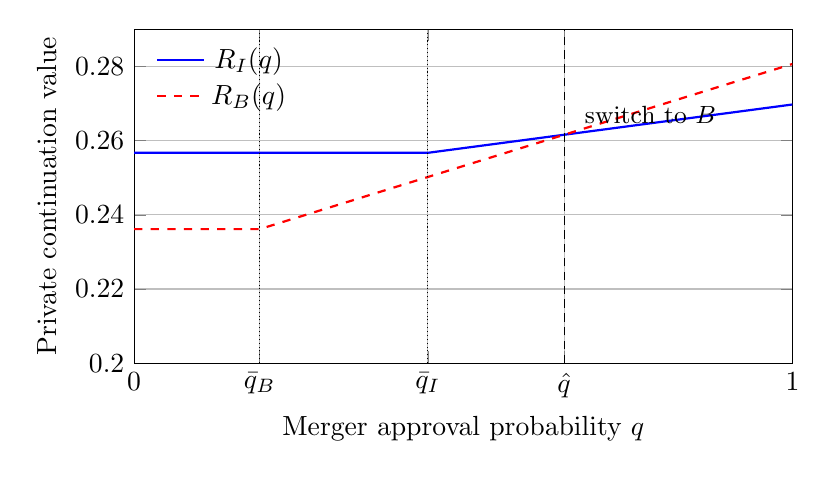
\begin{tikzpicture}
\begin{axis}[
    width=0.82\textwidth,
    height=0.48\textwidth,
    xmin=0, xmax=1,
    ymin=0.20, ymax=0.29,
    xlabel={Merger approval probability \(q\)},
    ylabel={Private continuation value},
    legend style={draw=none, fill=none, at={(0.02,0.98)}, anchor=north west},
    xtick={0,0.1907549041,0.4461335096,0.6531405543,1},
    xticklabels={0,\(\bar q_B\),\(\bar q_I\),\(\hat q\),1},
    ymajorgrids=true,
    xmajorgrids=true
]

\addplot[thick, blue] coordinates {
(0,0.2567111111)
(0.1,0.2567111111)
(0.1907549041,0.2567111111)
(0.3,0.2567111111)
(0.4461335096,0.2567111111)
(0.55,0.25915566668)
(0.6531405543,0.26158313693)
(0.8,0.26503955558)
(1,0.26974666670)
};
\addlegendentry{\(R_I(q)\)}

\addplot[thick, red, dashed] coordinates {
(0,0.2361313702)
(0.1,0.2361313702)
(0.1907549041,0.2361313702)
(0.3,0.24214470712)
(0.4461335096,0.25018854672)
(0.55,0.25590582122)
(0.6531405543,0.26158313696)
(0.8,0.26966693532)
(1,0.28067582660)
};
\addlegendentry{\(R_B(q)\)}

\addplot[densely dotted, black] coordinates {(0.1907549041,0.20) (0.1907549041,0.29)};
\addplot[densely dotted, black] coordinates {(0.4461335096,0.20) (0.4461335096,0.29)};
\addplot[densely dashed, black] coordinates {(0.6531405543,0.20) (0.6531405543,0.29)};

\node[anchor=south west] at (axis cs:0.67,0.262) {\small switch to \(B\)};
\end{axis}
\end{tikzpicture}
\caption{Illustrative private continuation values under the calibration reported in the text. The buyout-oriented project becomes privately optimal only after merger permissiveness passes the switching threshold \(\hat q\).}
\label{fig:continuation_values_calibrated}
\end{figure}

Finally, because \(s\) enters \eqref{eq:Uj} additively, the subsidy affects only the extensive margin.

\begin{corollary}\label{cor:subsidy}
For any given \(q\), the uniform entry subsidy \(s\) does not affect private project choice or effort.
It shifts the entry cutoff one-for-one:
\begin{equation}
    \frac{\partial f^*(s,q)}{\partial s}=1,
    \qquad
    \frac{\partial n(s,q)}{\partial s}=1.
\end{equation}
\end{corollary}

Corollary \ref{cor:subsidy} is useful for what follows.
The local government's uniform subsidy cannot redirect entrepreneurial effort across projects.
It can only expand or contract entry at the privately preferred project margin.
This irrelevance result is specific to a uniform, project-blind subsidy.
If policymakers could condition support on observable project orientation or on realized exit outcomes, project choice could in principle be affected; Section \ref{sec:extensions} illustrates that logic with a second, deliberately reduced-form instrument.
This is precisely why the interaction between merger policy and subsidy policy is central in the subsequent welfare analysis.

\section{Subsidy Design under Buyout Exit}\label{sec:subsidy}

This section derives the paper's main normative benchmark. The goal is to isolate the welfare consequences of buyout exit using only the product-market primitives introduced in Section \ref{sec:model} together with the endogenous merger-attempt condition. Planner-specific local and national incidence adjustments are postponed to Section \ref{sec:decentralized}.

\subsection{Primitive benchmark social value}

For project type $j\in\{I,B\}$, define the benchmark value under independent ownership by
\begin{equation}\label{eq:VjD}
    V_j^D \equiv C^D(j)+\pi_I^D(j)+\pi_E^D(j),
\end{equation}
and the benchmark value under approved acquisition by
\begin{equation}\label{eq:VjA}
    V_j^A \equiv C^M(j)+\Pi^M(j).
\end{equation}
Thus the benchmark welfare effect of approved acquisition relative to independent ownership is
\begin{equation}\label{eq:Omegaj}
    \Omega_j \equiv V_j^A-V_j^D.
\end{equation}
Using the definition of private merger surplus,
\begin{equation}\label{eq:Omegajdecomp}
    \Omega_j
    =
    \bigl(C^M(j)-C^D(j)\bigr)+\Delta_j.
\end{equation}
Equation \eqref{eq:Omegajdecomp} makes clear that the benchmark welfare effect of acquisition combines the private merger gain $\Delta_j$ with the product-market consumer-surplus effect.

Let
\begin{equation}
    a_j(q)\equiv \mathbf{1}\{q\Delta_j\ge k\}
\end{equation}
denote the merger-attempt indicator. The primitive-benchmark successful-project value is then
\begin{equation}\label{eq:BjPMq}
    B_j^{PM}(q)
    \equiv
    V_j^D+a_j(q)\bigl[q\Omega_j-k\bigr].
\end{equation}
This object is the benchmark welfare counterpart to the private continuation value in \eqref{eq:Rj}. If no merger is attempted, successful entry yields independent competition and therefore value $V_j^D$. If a merger is attempted, approved acquisition occurs with probability $q$, rejected merger with probability $1-q$, and the resource cost $k$ is incurred regardless of approval.

\subsection{Benchmark welfare conditional on project type}

Fix project type $j$. As in Section \ref{sec:private}, the entrepreneur chooses effort privately, so under Assumption \ref{ass:interior},
\begin{equation}
    x_j^*(q)=R_j(q),
    \qquad
    R_j(q)=\pi_E^D(j)+\beta[q\Delta_j-k]_+.
\end{equation}
For an entrepreneur with entry cost $f$, expected benchmark welfare from entering with project $j$ is therefore
\begin{equation}\label{eq:omegajPM}
    \omega_j^{PM}(f;s,q)
    =
    R_j(q)B_j^{PM}(q)
    -
    \frac{R_j(q)^2}{2}
    -
    f
    -
    \tau s.
\end{equation}
The private entry cutoff remains
\begin{equation}\label{eq:cjqPM}
    c_j(s,q)=s+\frac{R_j(q)^2}{2}.
\end{equation}
Hence benchmark welfare conditional on project $j$ is
\begin{equation}\label{eq:WjPM}
    W_j^{PM}(s,q)
    =
    \int_0^{c_j(s,q)}
    \left[
        R_j(q)B_j^{PM}(q)-\frac{R_j(q)^2}{2}-f-\tau s
    \right]df.
\end{equation}

\begin{proposition}\label{prop:pmbenchmarksubsidy}
Fix a project type $j\in\{I,B\}$ and an approval probability $q$. Then $W_j^{PM}(s,q)$ is strictly concave in $s$, and the unique optimal benchmark subsidy is
\begin{equation}\label{eq:sjPMstar}
    s_j^{PM*}(q)
    =
    \max\left\{
        0,\;
        \frac{
            R_j(q)B_j^{PM}(q)-\frac{\tau+2}{2}R_j(q)^2
        }{2\tau+1}
    \right\}.
\end{equation}
Equivalently,
\begin{equation}
    s_j^{PM*}(q)
    =
    \max\left\{
        0,\;
        \frac{
            R_j(q)\left[B_j^{PM}(q)-\frac{\tau+2}{2}R_j(q)\right]
        }{2\tau+1}
    \right\}.
\end{equation}
\end{proposition}

Proof is reported in Appendix \ref{app:decentralized}.

Proposition \ref{prop:pmbenchmarksubsidy} is the benchmark counterpart to the planner-specific subsidy formulas studied later. Its key feature is that the relevant welfare block is determined entirely by the product-market primitives together with the endogenous merger-attempt condition.

\subsection{Comparative statics under the primitive benchmark}

The first implication is that merger permissiveness matters only once a merger is privately attempted. If $q<\bar q_j\equiv k/\Delta_j$, then $a_j(q)=0$, so
\begin{equation}
    R_j(q)=\pi_E^D(j),
    \qquad
    B_j^{PM}(q)=V_j^D,
\end{equation}
and therefore the benchmark subsidy is locally constant in $q$.

\begin{proposition}\label{prop:pmcomparative}
Fix a project type $j\in\{I,B\}$.
\begin{enumerate}
    \item If $q<\bar q_j\equiv k/\Delta_j$, then $s_j^{PM*}(q)$ is constant in $q$.

    \item Consider an interval on which $q>\bar q_j$ and the optimal subsidy is interior. Then
    \begin{equation}\label{eq:dspmdq}
        \frac{d s_j^{PM*}(q)}{dq}
        =
        \frac{
            \beta\Delta_j\bigl[B_j^{PM}(q)-(\tau+2)R_j(q)\bigr]
            +
            R_j(q)\Omega_j
        }{2\tau+1}.
    \end{equation}

    \item In particular, if
    \begin{equation}\label{eq:pmnegativecase}
        \Omega_j\le 0
        \qquad\text{and}\qquad
        B_j^{PM}(q)\le (\tau+2)R_j(q),
    \end{equation}
    then
    \begin{equation}
        \frac{d s_j^{PM*}(q)}{dq}\le 0.
    \end{equation}
\end{enumerate}
\end{proposition}

Proof is reported in Appendix \ref{app:decentralized}.

Proposition \ref{prop:pmcomparative} isolates the model-driven comparative statics in a transparent way. The relevant objects are the private merger surplus $\Delta_j$, the benchmark social merger gain $\Omega_j$, and the private continuation value $R_j(q)$. No planner-specific incidence parameters appear in the theorem.

\subsection{Uniform subsidy under private project choice}

Return now to the actual equilibrium in which project choice is private and governed by Proposition \ref{prop:projectchoice}. Since the uniform subsidy does not affect project choice, the planner chooses $s$ taking $j^*(q)$ as given. Thus equilibrium benchmark welfare is
\begin{equation}
    W^{PM}(s,q)=W_{j^*(q)}^{PM}(s,q),
\end{equation}
and the optimal uniform benchmark subsidy is
\begin{equation}\label{eq:sPMuniform}
    s^{PM*}(q)=s_{j^*(q)}^{PM*}(q).
\end{equation}

\begin{proposition}\label{prop:pmuniformsubsidy}
Suppose Assumptions \ref{ass:types}--\ref{ass:singlecross} hold. Then the optimal uniform benchmark subsidy is
\begin{equation}
    s^{PM*}(q)
    =
    \begin{cases}
        s_I^{PM*}(q), & q<\hat q,\\
        \{s_I^{PM*}(\hat q),\, s_B^{PM*}(\hat q)\}, & q=\hat q,\\
        s_B^{PM*}(q), & q>\hat q.
    \end{cases}
\end{equation}
Moreover, if
\begin{equation}\label{eq:pmdropzero}
    B_B^{PM}(\hat q)<\frac{\tau+2}{2}R_B(\hat q),
\end{equation}
then there exists $\varepsilon>0$ such that
\begin{equation}
    s^{PM*}(q)=0
    \qquad
    \text{for all } q\in(\hat q,\hat q+\varepsilon).
\end{equation}
\end{proposition}

Proof is reported in Appendix \ref{app:decentralized}.

Proposition \ref{prop:pmuniformsubsidy} gives the paper's benchmark normative result. Merger permissiveness can redirect private project choice toward type $B$, and if the buyout-oriented project has weak benchmark social value relative to its private continuation value, the optimal subsidy falls and may vanish immediately after the project switch.

\subsection{Discussion}

The benchmark results in this section are driven by two primitive objects. The first is $\Delta_j$, which governs private merger feasibility and the private continuation value of entrepreneurship. The second is $\Omega_j=\Delta_j+\bigl(C^M(j)-C^D(j)\bigr)$, which governs the benchmark social gain from approved acquisition. This separation makes clear which comparative statics are model-driven before any planner-specific incidence assumptions are imposed.

Section \ref{sec:decentralized} builds on this benchmark by reintroducing local retention, planner-specific spillovers, and other incidence adjustments. Those planner-specific results therefore modify the benchmark derived here rather than replacing it.

\section{Incidence Extensions: Local versus National Policy}\label{sec:decentralized}

Section \ref{sec:subsidy} derived a primitive benchmark in which optimal subsidies and comparative statics are determined entirely by product-market primitives together with the endogenous merger-attempt condition. This section reintroduces planner-specific local retention and spillover incidence as adjustments around that benchmark. The comparison is not a strategic game across jurisdictions. For a fixed project type, the local--national difference is an incidence comparison around the primitive benchmark. What buyout exit adds is that the privately selected project can switch with merger permissiveness, thereby changing the relevant incidence comparison itself.

\subsection{Planner-specific incidence adjustments around the primitive benchmark}

Let $B_j^p(q)$ denote planner-$p$ successful-project value, and define the planner-specific incidence adjustment relative to the primitive benchmark by
\begin{equation}\label{eq:Djp}
    D_j^p(q)\equiv B_j^p(q)-B_j^{PM}(q).
\end{equation}
Planner-$p$ welfare conditional on project $j$ is
\begin{equation}\label{eq:Wjp}
    W_j^p(s,q)
    =
    \int_0^{c_j(s,q)}
    \left[
        R_j(q)B_j^p(q)-\frac{R_j(q)^2}{2}-f-\tau s
    \right]df,
\end{equation}
where the private entry cutoff remains
\begin{equation}
    c_j(s,q)=s+\frac{R_j(q)^2}{2}.
\end{equation}

\begin{proposition}\label{prop:incidencedecomp}
Fix a project type $j$ and an approval probability $q$. Let
\begin{equation}\label{eq:uPM}
    u_j^{PM}(q)
    \equiv
    \frac{
        R_j(q)B_j^{PM}(q)-\frac{\tau+2}{2}R_j(q)^2
    }{2\tau+1}.
\end{equation}
Then the planner-$p$ optimal subsidy is
\begin{equation}\label{eq:incidencedecomp}
    s_j^{p*}(q)
    =
    \max\left\{
        0,\;
        u_j^{PM}(q)+\frac{R_j(q)D_j^p(q)}{2\tau+1}
    \right\}.
\end{equation}
If, in addition, both the primitive benchmark subsidy and the planner-$p$ subsidy are interior at $(j,q)$, then
\begin{equation}\label{eq:incidencedecompinterior}
    s_j^{p*}(q)
    =
    s_j^{PM*}(q)
    +
    \frac{R_j(q)D_j^p(q)}{2\tau+1}.
\end{equation}
\end{proposition}

Proof is reported in Appendix \ref{app:decentralized}.

Proposition \ref{prop:incidencedecomp} places planner-specific incidence adjustments around the primitive benchmark in a way that remains valid globally once corner solutions are respected. The exact additive decomposition uses $s_j^{PM*}(q)$ only on interior regions where the primitive benchmark itself is not at the subsidy corner.

\subsection{Local and national planners as special cases}

For the local planner, let
\begin{align}
    B_j^{L,D}
    &\equiv
    C^D(j)
    + \lambda_I^L \pi_I^D(j)
    + \lambda_E^L \pi_E^D(j)
    + \eta_j^D, \label{eq:BLD} \\
    B_j^{L,A}
    &\equiv
    C^M(j)
    + \lambda_M^L \Pi^M(j)
    + \eta_j^A. \label{eq:BLA}
\end{align}
With local attempt-cost share $\kappa^L\in[0,1]$, successful-project value is
\begin{equation}\label{eq:BLq}
    B_j^L(q)
    =
    B_j^{L,D}
    +
    a_j(q)
    \left[
        q\bigl(B_j^{L,A}-B_j^{L,D}\bigr)-\kappa^L k
    \right].
\end{equation}
Appendix \ref{app:subsidy} develops useful decompositions for the local incidence block, including retained buyout proceeds and local spillover losses.

For the national planner, let
\begin{align}
    B_j^{N,D}
    &\equiv
    C^D(j)+\pi_I^D(j)+\pi_E^D(j)+\xi_j^D, \label{eq:BND} \\
    B_j^{N,A}
    &\equiv
    C^M(j)+\Pi^M(j)+\xi_j^A. \label{eq:BNA}
\end{align}
With national attempt-cost share $\kappa^N\in[0,1]$, successful-project value is
\begin{equation}\label{eq:BNq}
    B_j^N(q)
    =
    B_j^{N,D}
    +
    a_j(q)
    \left[
        q\bigl(B_j^{N,A}-B_j^{N,D}\bigr)-\kappa^N k
    \right].
\end{equation}
As special cases of \eqref{eq:Djp}, the local and national incidence adjustments are
\begin{equation}
    D_j^L(q)=B_j^L(q)-B_j^{PM}(q),
    \qquad
    D_j^N(q)=B_j^N(q)-B_j^{PM}(q).
\end{equation}

\begin{corollary}\label{cor:wedgefixed}
If both local and national optimal subsidies are interior, then for any fixed project type $j$,
\begin{equation}\label{eq:wedgefixed}
    s_j^{L*}(q)-s_j^{N*}(q)
    =
    \frac{R_j(q)\bigl(B_j^L(q)-B_j^N(q)\bigr)}{2\tau+1}.
\end{equation}
Hence the sign of the fixed-project wedge is the sign of $B_j^L(q)-B_j^N(q)$.
\end{corollary}

Proof is reported in Appendix \ref{app:decentralized}.

Corollary \ref{cor:wedgefixed} shows that once the primitive benchmark has been isolated, the fixed-project local--national wedge is an algebraic incidence comparison. Appendices \ref{app:sufficientlocalover} and \ref{app:sufficientlocalunder} give sufficient conditions for positive and negative wedges in terms of retained buyout proceeds and locally concentrated post-acquisition losses.

\subsection{Equilibrium wedges under private project choice}

Reintroduce private project choice. Let
\begin{equation}
    j^*(q)\in\{I,B\}
\end{equation}
denote the entrepreneur's privately optimal project and define
\begin{equation}
    \bar R(q)\equiv R_{j^*(q)}(q),
    \qquad
    \bar B^L(q)\equiv B_{j^*(q)}^L(q),
    \qquad
    \bar B^N(q)\equiv B_{j^*(q)}^N(q).
\end{equation}

\begin{corollary}\label{cor:wedgeequilibrium}
Suppose Assumptions \ref{ass:types}--\ref{ass:singlecross} hold and both planner-specific subsidies are interior on the relevant range. Then
\begin{equation}\label{eq:wedgeequilibrium}
    s^{L*}(q)-s^{N*}(q)
    =
    \frac{\bar R(q)\bigl(\bar B^L(q)-\bar B^N(q)\bigr)}{2\tau+1}.
\end{equation}
In particular, if
\begin{equation}
    B_I^L(q)<B_I^N(q)
    \quad\text{for } q<\hat q,
    \qquad\text{and}\qquad
    B_B^L(q)>B_B^N(q)
    \quad\text{for } q>\hat q,
\end{equation}
then the sign of the equilibrium subsidy wedge changes at the project-switching threshold.
\end{corollary}

Proof is reported in Appendix \ref{app:decentralized}.

For illustration, Figures \ref{fig:local_national_subsidies_calibrated}--\ref{fig:wedge_calibrated}
use the following parameterization:
\[
a_I=1.2,\quad \sigma_I=0.5,\quad m_I=0.05,
\qquad
a_B=1.1,\quad \sigma_B=0.3,\quad m_B=0.15,
\]
\[
\beta=0.35,\quad k=0.03,\quad \tau=1,
\]
together with
\[
\lambda_I^L=0.2,\quad \lambda_E^L=0.7,\quad \lambda_M^L=0.15,
\]
\[
\eta_I^D=0.10,\quad \eta_I^A=0.05,\quad \eta_B^D=0.08,\quad \eta_B^A=0.02,
\]
\[
\xi_I^D=0.12,\quad \xi_I^A=0.08,\quad \xi_B^D=0.10,\quad \xi_B^A=0.04,
\qquad
\kappa^L=\kappa^N=1.
\]
These values imply
\[
\bar q_B \approx 0.1908,\qquad
\bar q_I \approx 0.4461,\qquad
\hat q \approx 0.6531.
\]
The calibration is chosen only to illustrate the qualitative comparative statics and threshold ordering of the model; it is not intended as a quantitative fit to any specific institutional setting.

\begin{figure}[t]
\centering
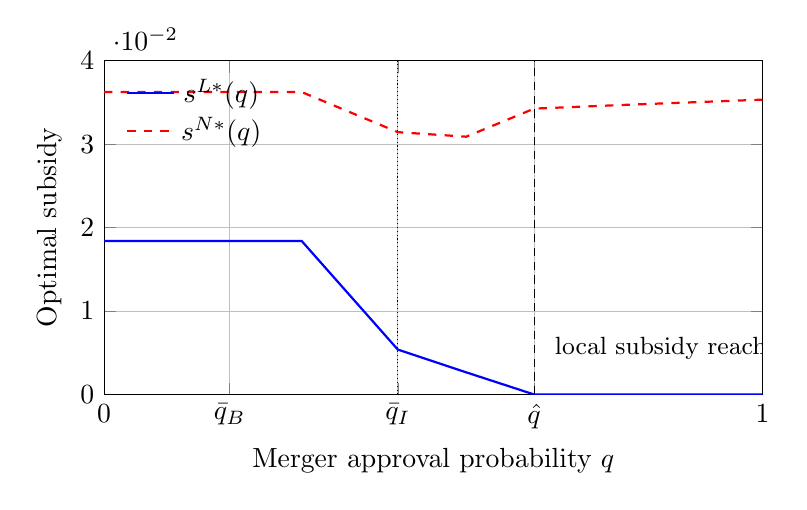
\begin{tikzpicture}
\begin{axis}[
    width=0.82\textwidth,
    height=0.48\textwidth,
    xmin=0, xmax=1,
    ymin=0, ymax=0.04,
    xlabel={Merger approval probability \(q\)},
    ylabel={Optimal subsidy},
    legend style={draw=none, fill=none, at={(0.02,0.98)}, anchor=north west},
    xtick={0,0.1907549041,0.4461335096,0.6531405543,1},
    xticklabels={0,\(\bar q_B\),\(\bar q_I\),\(\hat q\),1},
    ymajorgrids=true,
    xmajorgrids=true
]

\addplot[thick, blue] coordinates {
(0,0.01840865870)
(0.1,0.01840865870)
(0.1907549041,0.01840865870)
(0.3,0.01840865870)
(0.4461335096,0.00538027289)
(0.55,0.00265601444)
(0.6531405543,0)
(0.8,0)
(1,0)
};
\addlegendentry{\(s^{L*}(q)\)}

\addplot[thick, red, dashed] coordinates {
(0,0.03625141202)
(0.1,0.03625141202)
(0.1907549041,0.03625141202)
(0.3,0.03625141202)
(0.4461335096,0.03144295670)
(0.55,0.03089882779)
(0.6531405543,0.03426378692)
(0.8,0.03474278419)
(1,0.03533919386)
};
\addlegendentry{\(s^{N*}(q)\)}

\addplot[densely dotted, black] coordinates {(0.4461335096,0) (0.4461335096,0.04)};
\addplot[densely dashed, black] coordinates {(0.6531405543,0) (0.6531405543,0.04)};

\node[anchor=south west] at (axis cs:0.67,0.003) {\small local subsidy reaches zero};
\end{axis}
\end{tikzpicture}
\caption{Illustrative local and national optimal subsidies under the calibration reported in the text. The figure plots the constrained planner-specific optima, including the subsidy corner at zero. Accordingly, the interior closed-form expressions that underlie Corollaries \ref{cor:wedgefixed} and \ref{cor:wedgeequilibrium} apply only on subregions where the relevant planner-specific subsidies remain strictly positive. In this calibration, easier buyout exit weakens the case for local subsidy, and the local planner withdraws support after the switch to buyout-oriented entrepreneurship.}
\label{fig:local_national_subsidies_calibrated}
\end{figure}

\begin{figure}[t]
\centering
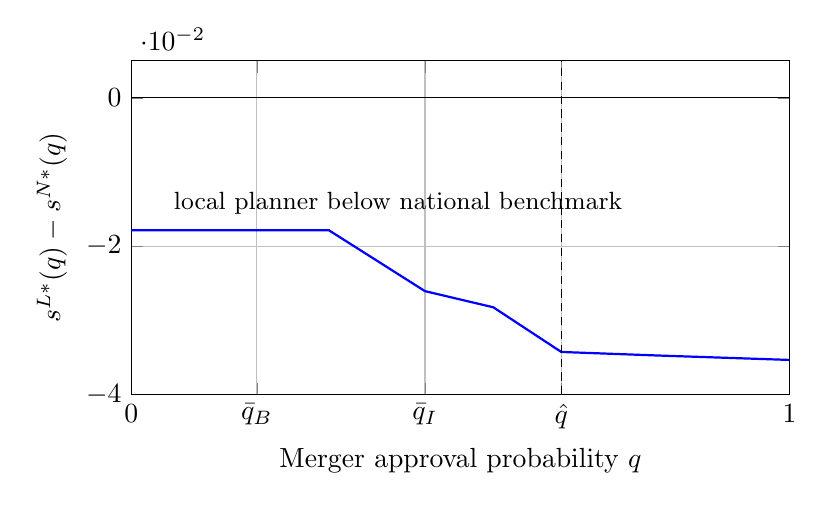
\begin{tikzpicture}
\begin{axis}[
    width=0.82\textwidth,
    height=0.48\textwidth,
    xmin=0, xmax=1,
    ymin=-0.04, ymax=0.005,
    xlabel={Merger approval probability \(q\)},
    ylabel={\(s^{L*}(q)-s^{N*}(q)\)},
    xtick={0,0.1907549041,0.4461335096,0.6531405543,1},
    xticklabels={0,\(\bar q_B\),\(\bar q_I\),\(\hat q\),1},
    ymajorgrids=true,
    xmajorgrids=true
]

\addplot[thick, blue] coordinates {
(0,-0.01784275331)
(0.1,-0.01784275331)
(0.1907549041,-0.01784275331)
(0.3,-0.01784275331)
(0.4461335096,-0.02606268381)
(0.55,-0.02824281335)
(0.6531405543,-0.03426378692)
(0.8,-0.03474278419)
(1,-0.03533919386)
};
\addplot[thin, black] coordinates {(0,0) (1,0)};
\addplot[densely dashed, black] coordinates {(0.6531405543,-0.04) (0.6531405543,0.005)};

\node[anchor=south west] at (axis cs:0.05,-0.017) {\small local planner below national benchmark};
\end{axis}
\end{tikzpicture}
\caption{Illustrative local--national incidence wedge around the primitive benchmark under the calibration reported in the text. The plotted wedge is the difference between the constrained optimal subsidies from Figure \ref{fig:local_national_subsidies_calibrated}. Hence, once one planner hits the zero-subsidy corner, the plotted wedge need not coincide with the interior formula in Corollary \ref{cor:wedgeequilibrium}. In this benchmark-consistent calibration, the local planner values successful entrepreneurial entry less than the national planner throughout, so the wedge remains negative even though its magnitude changes discretely when project choice switches.}
\label{fig:wedge_calibrated}
\end{figure}

\subsection{Discussion}

Section \ref{sec:subsidy} established that the main subsidy comparative statics are first pinned down by the primitive benchmark objects $\Delta_j$ and $\Omega_j$. The local and national results here are planner-specific adjustments around that benchmark.

This ordering clarifies the interpretation of the wedge results. For a fixed project, the sign of the local--national difference is an incidence comparison. What buyout exit adds is that merger permissiveness can change the privately selected project, thereby changing the economically relevant incidence comparison. Appendix Figure \ref{fig:wedge_sign_reversal_appendix} reports a transfer-augmented calibration illustrating the sign-reversal case highlighted in Corollary \ref{cor:wedgeequilibrium}.

\section{Illustrative Extension: Clawbacks and Policy Design}\label{sec:extensions}

Sections \ref{sec:subsidy} and \ref{sec:decentralized} contain the paper's core analytical contribution. This section is deliberately illustrative: it introduces a second instrument only to show, in reduced form, how policy design could target the composition margin created by buyout exit. A uniform entry subsidy affects only the extensive margin. It cannot alter private project choice and therefore cannot correct that distortion on its own.

\subsection{A buyout-contingent clawback}

We model the clawback as a reduced-form tax on the entrepreneur's merger-related continuation payoff. The goal is to isolate the composition effect of reducing the entrepreneur's private reward from sell-out-oriented innovation while holding fixed the merger technology and product-market consequences of acquisition.

\begin{assumption}\label{ass:clawback}
The clawback redistributes merger-related gains away from the entrepreneur without changing the joint surplus from attempting a merger, the merger technology itself, or the realized product-market outcome conditional on approval.
\end{assumption}
This is a maintained invariance assumption used to keep the extension transparent; it is not intended as a complete institutional description of all clawback arrangements.

Under Assumption \ref{ass:clawback}, the merger-attempt condition remains
\begin{equation}\label{eq:attemptconditionrho}
    q\Delta_j \ge k,
\end{equation}
so the attempt indicator is unchanged:
\begin{equation}
    a_j(q)=\mathbf{1}\{q\Delta_j \ge k\}.
\end{equation}
Because realized product-market outcomes and merger feasibility are unchanged, the welfare objects \(B_j^L(q)\) and \(B_j^N(q)\) remain those defined earlier. The clawback operates only through private continuation values and the induced changes in effort, entry, and project choice.

If the entrepreneur must remit a fraction \(\rho \in [0,1)\) of merger-related continuation gains, then conditional on success and project choice \(j\), private continuation value becomes
\begin{equation}\label{eq:Rtilde}
    \widetilde R_j(q,\rho)
    =
    \pi_E^D(j)
    +
    (1-\rho)\beta [q\Delta_j-k]_+.
\end{equation}
Under the corresponding interiority condition,
\begin{equation}
    \widetilde x_j^*(q,\rho)=\widetilde R_j(q,\rho),
    \qquad
    \widetilde U_j(f;s,q,\rho)=s-f+\frac{\widetilde R_j(q,\rho)^2}{2}.
\end{equation}
Define
\begin{equation}
    \widetilde A_j(q,\rho)\equiv \frac{\widetilde R_j(q,\rho)^2}{2},
    \qquad
    \widetilde c_j(s,q,\rho)\equiv s+\widetilde A_j(q,\rho).
\end{equation}
Then the mass of entrants under project \(j\) is \(\widetilde n_j(s,q,\rho)=\widetilde c_j(s,q,\rho)\).

\begin{proposition}\label{prop:clawbackthreshold}
Suppose Assumptions \ref{ass:types} and \ref{ass:singlecross} hold, and consider values of \(q\) such that both project types are merger-feasible. Then there exists a unique project-switching threshold
\begin{equation}\label{eq:qhatrho}
    \hat q(\rho)
    =
    \frac{
        \pi_E^D(I)-\pi_E^D(B)
    }{
        (1-\rho)\beta(\Delta_B-\Delta_I)
    }.
\end{equation}
The entrepreneur chooses the buyout-oriented project if and only if \(q>\hat q(\rho)\), and
\begin{equation}\label{eq:dqhatdrho}
    \frac{\partial \hat q(\rho)}{\partial \rho}
    =
    \frac{\hat q(\rho)}{1-\rho}
    >0.
\end{equation}
\end{proposition}

A higher clawback therefore makes buyout-oriented innovation less attractive by shifting the switching threshold to the right. For any fixed approval probability \(q\), the minimal clawback required to restore the independence-oriented project is
\begin{equation}\label{eq:rhobar}
    \bar \rho(q)
    \equiv
    \max\left\{
        0,\;
        1-
        \frac{
            \pi_E^D(I)-\pi_E^D(B)
        }{
            \beta q(\Delta_B-\Delta_I)
        }
    \right\},
\end{equation}
provided both projects are merger-feasible.

Figure \ref{fig:clawback_threshold_calibrated} illustrates this threshold effect under the benchmark calibration.

\begin{figure}[t]
\centering
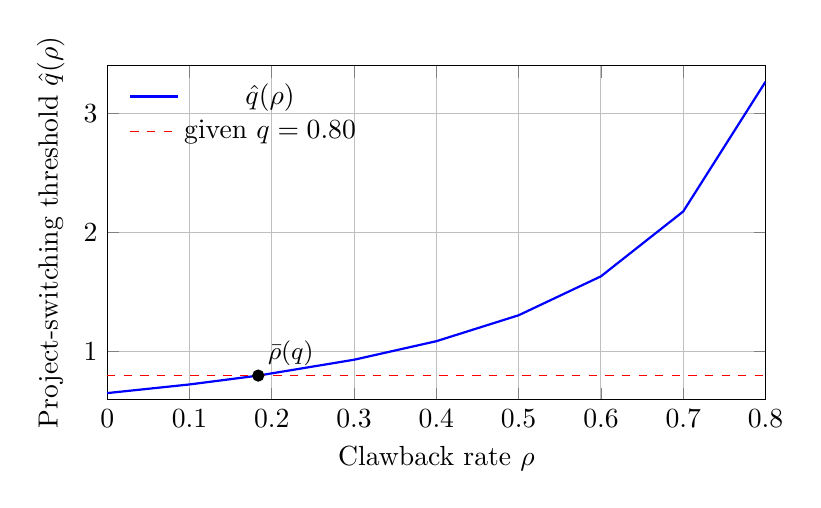
\begin{tikzpicture}
\begin{axis}[
    width=0.82\textwidth,
    height=0.48\textwidth,
    xmin=0, xmax=0.8,
    ymin=0.60, ymax=3.4,
    xlabel={Clawback rate \(\rho\)},
    ylabel={Project-switching threshold \(\hat q(\rho)\)},
    legend style={draw=none, fill=none, at={(0.02,0.98)}, anchor=north west},
    ymajorgrids=true,
    xmajorgrids=true
]

\addplot[thick, blue] coordinates {
(0,0.6531405543)
(0.1,0.7257117270)
(0.1835743071,0.8000000000)
(0.3,0.9330579347)
(0.4,1.0885675905)
(0.5,1.3062811086)
(0.6,1.6328513858)
(0.7,2.1771351810)
(0.8,3.2657027715)
};
\addlegendentry{\(\hat q(\rho)\)}

\addplot[red, dashed] coordinates {(0,0.80) (0.8,0.80)};
\addlegendentry{given \(q=0.80\)}

\addplot[only marks, mark=*, mark size=2pt] coordinates {(0.1835743071,0.80)};
\node[anchor=south west] at (axis cs:0.1836,0.80) {\small \(\bar\rho(q)\)};

\end{axis}
\end{tikzpicture}
\caption{Illustrative effect of a buyout-contingent clawback on the project-switching threshold under the calibration reported in the text. Since \(\hat q(\rho)\) increases in \(\rho\), a higher clawback makes buyout-oriented innovation less attractive for any given approval probability \(q\).}
\label{fig:clawback_threshold_calibrated}
\end{figure}

\subsection{Subsidy formulas under a clawback}

Because the clawback changes private continuation values but not welfare incidence for a given realized outcome, the local planner's type-\(j\) welfare becomes
\begin{equation}\label{eq:WtildeL}
    \widetilde W_j^L(s,q,\rho)
    =
    \widetilde c_j(s,q,\rho)
    \left(
        \widetilde R_j(q,\rho)B_j^L(q)
        -
        \widetilde A_j(q,\rho)
        -
        \tau s
    \right)
    -
    \frac{\widetilde c_j(s,q,\rho)^2}{2},
\end{equation}
with optimal subsidy
\begin{equation}\label{eq:stildeclaw}
    \widetilde s_j^{L*}(q,\rho)
    =
    \max\left\{
        0,\;
        \frac{
            \widetilde R_j(q,\rho)B_j^L(q)
            -
            \frac{\tau+2}{2}\widetilde R_j(q,\rho)^2
        }{2\tau+1}
    \right\}.
\end{equation}
Similarly,
\begin{equation}\label{eq:stildeclawn}
    \widetilde s_j^{N*}(q,\rho)
    =
    \max\left\{
        0,\;
        \frac{
            \widetilde R_j(q,\rho)B_j^N(q)
            -
            \frac{\tau+2}{2}\widetilde R_j(q,\rho)^2
        }{2\tau+1}
    \right\}.
\end{equation}
Whenever both are interior,
\begin{equation}\label{eq:wedgeclawback}
    \widetilde s_j^{L*}(q,\rho)-\widetilde s_j^{N*}(q,\rho)
    =
    \frac{
        \widetilde R_j(q,\rho)\bigl(B_j^L(q)-B_j^N(q)\bigr)
    }{2\tau+1}.
\end{equation}
Thus the clawback rescales the magnitude of the local--national wedge for a given project type, while potentially changing the equilibrium wedge indirectly through project switching.

\subsection{Illustrative joint design with merger policy}

Let \(\theta\) denote a policy shifter of \(q\), with antitrust toughness as one interpretation:
\begin{equation}
    q=q(\theta),
    \qquad
    q'(\theta)<0.
\end{equation}
Under a clawback, project \(B\) is privately chosen whenever \(q(\theta)>\hat q(\rho)\). Hence the set of policy pairs \((\theta,\rho)\) that leave the entrepreneur indifferent between projects satisfies
\begin{equation}\label{eq:implementationlocus}
    q(\theta)=\hat q(\rho).
\end{equation}

\begin{proposition}\label{prop:instrumentsubstitution}
Suppose \(q'(\theta)<0\), and consider the locus of policy pairs \((\theta,\rho)\) satisfying \eqref{eq:implementationlocus}. Then:
\begin{enumerate}
    \item A higher clawback rate \(\rho\) permits a lower antitrust toughness \(\theta\) while keeping project choice unchanged.
    \item The independence-oriented project can be implemented by stricter merger policy, a stronger clawback, or a combination of the two.
    \item Along the implementation locus,
    \begin{equation}\label{eq:dthetadrho}
        \frac{d\theta}{d\rho}
        =
        \frac{\hat q'(\rho)}{q'(\theta)}
        <0.
    \end{equation}
\end{enumerate}
\end{proposition}

Within this illustrative extension, clawbacks and merger policy are therefore substitute instruments for the composition margin. A stronger clawback reduces private sell-out incentives directly, whereas stricter merger policy does so indirectly by lowering the probability of approved acquisition.

\subsection{Illustrative policy-design implications}

The extension reinforces a simple policy-design lesson. Uniform entry subsidies are useful for the extensive margin but poorly suited to environments in which the main concern is the \emph{type} of startups being created. A buyout-contingent clawback adds a second instrument that directly targets composition. In the present framework,
\begin{itemize}
    \item the subsidy \(s\) governs how many entrepreneurs enter,
    \item the clawback \(\rho\) governs how attractive buyout-oriented innovation is relative to independence-oriented innovation, and
    \item merger policy \(q\) or \(\theta\) governs the overall exit environment.
\end{itemize}
This separation of instruments is especially relevant when local and national planners value acquisition-oriented entrepreneurship differently, but the discussion here should be read as a proof-of-concept extension rather than as the paper's central institutional result.

\section{Conclusion}\label{sec:conclusion}

This paper studies startup subsidies in an environment in which entrepreneurial success often leads to acquisition rather than independent competition. Prospective entrepreneurs choose whether to enter, how much effort to exert, and whether to pursue an independence-oriented or a buyout-oriented project. After success, the entrant may be acquired by an incumbent, subject to merger approval, and a government chooses an entry subsidy before entry takes place.

The analysis yields three main results. First, a more permissive exit environment raises the private continuation value of entrepreneurship and therefore increases entry and effort. Second, it can redirect entrepreneurial project choice toward projects that are attractive primarily because they generate large acquisition premia rather than because they create strong stand-alone competitors. Third, because a uniform entry subsidy does not affect project choice, it cannot correct this composition distortion. Easier buyout exit need not strengthen the case for startup support and can instead reduce the optimal subsidy.

A central methodological implication is that welfare analysis must respect the same behavioral margins that govern private equilibrium. A merger is attempted only when expected private merger gains cover filing and implementation costs, so the social value of successful entry cannot be written as a simple convex combination of independent ownership and approved acquisition. In the paper's benchmark analysis, the resulting subsidy formulas and comparative statics are derived first from product-market primitives and the endogenous merger-attempt condition alone. Once this distinction is imposed, merger policy affects subsidy design only when it changes actual behavior.

The paper also characterizes a local--national incidence wedge. Local and national authorities may value successful entrepreneurial projects differently because the incidence of gains and losses from acquisition differs across levels of government. In the revised presentation, those local and national results are derived as planner-specific incidence adjustments around the primitive benchmark. For a fixed project, the local--national difference is therefore an incidence comparison. What buyout exit adds is that the privately selected project can itself change with merger permissiveness, so the economically relevant local--national comparison can change as well. Local governments may therefore subsidize too much or too little relative to the national benchmark even when both policymakers face the same private equilibrium.

The broader implication is that startup subsidies and merger policy should not be studied in isolation. Entry subsidies govern the scale of entrepreneurship, but the exit environment shapes private project direction. When acquisition is an important exit route, policy design requires instruments that address both margins. A final, explicitly exploratory implication concerns policy design beyond the baseline model: buyout-contingent clauses, such as clawbacks tied to acquisition, can complement uniform subsidies by affecting not only how much entrepreneurship occurs but also what type of entrepreneurship is pursued. This extension is intended to illustrate instrument separation rather than to displace the paper's main analytical contribution, which lies in the behaviorally consistent welfare analysis of Sections \ref{sec:subsidy} and \ref{sec:decentralized}.

The model is intentionally stylized. Natural extensions include richer merger review, multiple entrants, dynamic innovation races, and explicit multi-jurisdiction competition. The present paper, however, studies incidence-based divergence between local and national policy rather than strategic interaction across jurisdictions. Even so, the main message is simple: in economies where acquisition is a central entrepreneurial exit route, startup policy is not only about creating more firms. It is also about shaping what kinds of firms are created and how the gains and losses from their exit are distributed across policymakers.


\appendix
\section{Omitted derivations for Section \ref{sec:model}}\label{app:modelderivations}

\subsection{Independent Cournot equilibrium}

Fix a project type \(j \in \{I,B\}\), and suppress the type index for notational convenience.
Under independent ownership, the incumbent and the entrant solve
\begin{align}
    \max_{q_I \ge 0}\;& (1-q_I-\sigma q_E)q_I, \\
    \max_{q_E \ge 0}\;& (a-q_E-\sigma q_I)q_E.
\end{align}
The first-order conditions are
\begin{align}
    1-2q_I-\sigma q_E &= 0, \\
    a-2q_E-\sigma q_I &= 0.
\end{align}
Solving the linear system yields
\begin{align}
    q_I^D &= \frac{2-a\sigma}{4-\sigma^2}, \\
    q_E^D &= \frac{2a-\sigma}{4-\sigma^2}.
\end{align}
Substituting these quantities into inverse demand gives
\begin{align}
    p_I^D &= 1-q_I^D-\sigma q_E^D = q_I^D, \\
    p_E^D &= a-q_E^D-\sigma q_I^D = q_E^D.
\end{align}
Hence independent profits are
\begin{align}
    \pi_I^D &= (q_I^D)^2
    = \left(\frac{2-a\sigma}{4-\sigma^2}\right)^2, \\
    \pi_E^D &= (q_E^D)^2
    = \left(\frac{2a-\sigma}{4-\sigma^2}\right)^2.
\end{align}

\subsection{Merged-firm outcome}

Under common ownership, the merged firm chooses \((q_I,q_E)\) to maximize
\begin{equation}
    (1-q_I-\sigma q_E)q_I + (a-q_E-\sigma q_I)q_E + m.
\end{equation}
The first-order conditions are
\begin{align}
    1-2q_I-2\sigma q_E &= 0, \\
    a-2q_E-2\sigma q_I &= 0.
\end{align}
Solving yields
\begin{align}
    q_I^M &= \frac{1-a\sigma}{2(1-\sigma^2)}, \\
    q_E^M &= \frac{a-\sigma}{2(1-\sigma^2)}.
\end{align}
Substituting into joint operating profit yields
\begin{equation}
    \Pi_{\mathrm{op}}^M
    =
    \frac{a^2-2a\sigma+1}{4(1-\sigma^2)}.
\end{equation}
Therefore total merged profit is
\begin{equation}
    \Pi^M
    =
    \frac{a^2-2a\sigma+1}{4(1-\sigma^2)} + m.
\end{equation}
The merger surplus is
\begin{equation}
    \Delta
    =
    \Pi^M-\pi_I^D-\pi_E^D.
\end{equation}

\subsection{Consumer surplus}

A quadratic utility representation that rationalizes the inverse demands in Section \ref{sec:model} is
\begin{equation}
    U(q_I,q_E)
    =
    y + q_I + a q_E
    - \frac{1}{2}
      \left(
        q_I^2 + 2\sigma q_I q_E + q_E^2
      \right),
\end{equation}
where \(y\) is numeraire consumption.
Inverse demands are the marginal utilities:
\begin{align}
    p_I &= \frac{\partial U}{\partial q_I}
    = 1-q_I-\sigma q_E, \\
    p_E &= \frac{\partial U}{\partial q_E}
    = a-q_E-\sigma q_I.
\end{align}
Hence consumer surplus is
\begin{equation}
    C(q_I,q_E)
    =
    \frac{1}{2}
    \left(
        q_I^2 + q_E^2 + 2\sigma q_I q_E
    \right).
\end{equation}
Evaluating this expression at \((q_I^D,q_E^D)\) and \((q_I^M,q_E^M)\) yields \(C^D(j)\) and \(C^M(j)\), respectively.

\subsection{Merger-attempt threshold}

For a successful type-\(j\) project, the joint payoff from attempting a merger is
\begin{equation}
    q\Pi^M(j) + (1-q)\bigl(\pi_I^D(j)+\pi_E^D(j)\bigr) - k.
\end{equation}
The joint payoff from not attempting a merger is
\begin{equation}
    \pi_I^D(j)+\pi_E^D(j).
\end{equation}
Therefore a merger is attempted if and only if
\begin{equation}
    q\Pi^M(j) + (1-q)\bigl(\pi_I^D(j)+\pi_E^D(j)\bigr) - k
    \ge
    \pi_I^D(j)+\pi_E^D(j),
\end{equation}
which simplifies to
\begin{equation}
    q\Delta_j \ge k.
\end{equation}
This yields the attempt indicator
\begin{equation}
    a_j(q)=\mathbf{1}\{q\Delta_j \ge k\}
\end{equation}
used in Sections \ref{sec:subsidy} and \ref{sec:decentralized}.

\subsection*{A.5 Welfare accounting and the primitive benchmark}

The main text distinguishes between the approval probability \(q\) and the attempt decision
\begin{equation}
    a_j(q)=\mathbf{1}\{q\Delta_j\ge k\}.
\end{equation}
This distinction is essential for consistent welfare accounting.

If \(q\Delta_j<k\), then no merger is attempted in private equilibrium. In that case, successful
entry necessarily results in independent competition, so any successful-project welfare object must
coincide with the corresponding independent-ownership value.

If \(q\Delta_j\ge k\), then a merger is attempted. Conditional on attempt, approved acquisition
occurs with probability \(q\), rejected merger with probability \(1-q\), and the real resource cost \(k\)
is incurred regardless of approval. This is why planner-specific successful-project values in the main
text take the piecewise form
\begin{equation}
    B_j^p(q)=B_j^{p,D}+a_j(q)\Bigl[q\bigl(B_j^{p,A}-B_j^{p,D}\bigr)-\kappa^p k\Bigr],
\end{equation}
where \(p\) indexes the planner.

For the primitive benchmark introduced in revised Section \ref{sec:subsidy}, define
\begin{equation}
    V_j^D \equiv C^D(j)+\pi_I^D(j)+\pi_E^D(j),
    \qquad
    V_j^A \equiv C^M(j)+\Pi^M(j),
\end{equation}
and
\begin{equation}
    \Omega_j \equiv V_j^A-V_j^D.
\end{equation}
Using the definition of private merger surplus,
\begin{equation}
    \Delta_j=\Pi^M(j)-\pi_I^D(j)-\pi_E^D(j),
\end{equation}
we can write
\begin{equation}
    \Omega_j
    =
    \bigl(C^M(j)-C^D(j)\bigr)+\Delta_j.
\end{equation}
Hence the primitive benchmark successful-project value is
\begin{equation}
    B_j^{PM}(q)\equiv V_j^D+a_j(q)\bigl[q\Omega_j-k\bigr].
\end{equation}
This benchmark uses only product-market primitives together with the same endogenous merger-attempt
condition that governs private continuation values.

\section{Appendix to Section \ref{sec:private}}\label{app:privateproofs}

\subsection{Effort choice}\label{app:effort}

For a given project type \(j\), the entrepreneur solves
\begin{equation}
    \max_{x \in [0,1]}
    \left\{
        xR_j(q)-\frac{x^2}{2}
    \right\}.
\end{equation}
The derivative is
\begin{equation}
    \frac{\partial}{\partial x}
    \left(
        xR_j(q)-\frac{x^2}{2}
    \right)
    =
    R_j(q)-x.
\end{equation}
Hence the unconstrained optimum is \(x=R_j(q)\).
Imposing the constraint \(x \in [0,1]\) yields
\begin{equation}\label{eq:xgeneral}
    x_j^*(q)=\min\{R_j(q),1\},
\end{equation}
since \(R_j(q)>0\).
Under Assumption \ref{ass:interior}, \(R_j(q)\in(0,1)\), so \eqref{eq:xgeneral} reduces to \eqref{eq:xjstar}.

Substituting \(x_j^*(q)=R_j(q)\) into the entrepreneur's objective yields
\begin{equation}
    \max_{x \in [0,1]}
    \left\{
        xR_j(q)-\frac{x^2}{2}
    \right\}
    =
    \frac{R_j(q)^2}{2},
\end{equation}
which gives \eqref{eq:Uj}.

\subsection{Project choice without the single-crossing restriction}\label{app:projchoice}

Define the private payoff difference
\begin{equation}
    D(q)\equiv R_B(q)-R_I(q).
\end{equation}
Using the definition of \(R_j(q)\), this difference is
\begin{equation}\label{eq:Dqpiece}
    D(q)
    =
    \begin{cases}
        \pi_E^D(B)-\pi_E^D(I), &
        q < \bar q_B, \\
        \pi_E^D(B)-\pi_E^D(I)+\beta(q\Delta_B-k), &
        \bar q_B \le q < \bar q_I, \\
        \pi_E^D(B)-\pi_E^D(I)+\beta q(\Delta_B-\Delta_I), &
        q \ge \bar q_I.
    \end{cases}
\end{equation}
Because \(\pi_E^D(I)>\pi_E^D(B)\), we have \(D(q)<0\) for all \(q<\bar q_B\).
In the intermediate region \([\bar q_B,\bar q_I)\), the buyout-oriented project is preferred if and only if
\begin{equation}\label{eq:qtilde}
    q \ge \tilde q
    \equiv
    \frac{\pi_E^D(I)-\pi_E^D(B)+\beta k}{\beta \Delta_B}.
\end{equation}
Once both projects are merger-feasible, the buyout-oriented project is preferred if and only if
\begin{equation}\label{eq:qhatappendix}
    q \ge \hat q
    \equiv
    \frac{\pi_E^D(I)-\pi_E^D(B)}{\beta(\Delta_B-\Delta_I)}.
\end{equation}

Assumption \ref{ass:singlecross} implies \(\hat q \ge \bar q_I\).
This is equivalent to
\begin{equation}
    \pi_E^D(I)-\pi_E^D(B)
    \ge
    \beta k\left(\frac{\Delta_B}{\Delta_I}-1\right),
\end{equation}
which in turn implies \(\tilde q \ge \bar q_I\).
Hence no switching occurs in the intermediate region \([\bar q_B,\bar q_I)\), and the equilibrium project choice collapses to the single-threshold characterization in Proposition \ref{prop:projectchoice}.

\subsection{Proof of Proposition \ref{prop:projectchoice}}

By \eqref{eq:Dqpiece}, the payoff difference \(D(q)=R_B(q)-R_I(q)\) is weakly increasing in \(q\), and strictly increasing on any interval where at least one project is merger-feasible.

For \(q<\bar q_I\), Assumption \ref{ass:singlecross} and Appendix \ref{app:projchoice} imply \(D(q)<0\), so project \(I\) is privately optimal.

For \(q\ge \bar q_I\), both projects are merger-feasible and
\begin{equation}
    D(q)
    =
    \pi_E^D(B)-\pi_E^D(I)+\beta q(\Delta_B-\Delta_I).
\end{equation}
Because \(\Delta_B>\Delta_I\), this expression is strictly increasing in \(q\), and it equals zero at
\begin{equation}
    q=\hat q
    =
    \frac{\pi_E^D(I)-\pi_E^D(B)}
         {\beta(\Delta_B-\Delta_I)}.
\end{equation}
Assumption \ref{ass:singlecross} ensures \(\hat q \in [\bar q_I,1)\).
Therefore \(D(q)<0\) for \(q<\hat q\), \(D(q)=0\) at \(q=\hat q\), and \(D(q)>0\) for \(q>\hat q\), proving Proposition \ref{prop:projectchoice}. \qed

\subsection{Proof of Proposition \ref{prop:entrymonotonicity}}

By \eqref{eq:Rbarpiece},
\begin{equation}
    \bar R(q)
    =
    \begin{cases}
        \pi_E^D(I), &
        q < \bar q_I, \\
        \pi_E^D(I)+\beta(q\Delta_I-k), &
        \bar q_I \le q < \hat q, \\
        \pi_E^D(B)+\beta(q\Delta_B-k), &
        q \ge \hat q.
    \end{cases}
\end{equation}
Differentiating on each interval yields
\begin{equation}
    \frac{d\bar R(q)}{dq}
    =
    \begin{cases}
        0, & q < \bar q_I, \\
        \beta \Delta_I, & \bar q_I < q < \hat q, \\
        \beta \Delta_B, & q > \hat q,
    \end{cases}
\end{equation}
which proves part (i).

Part (ii) follows from \(x^*(q)=\bar R(q)\).

For part (iii), recall that under Assumption \ref{ass:interior},
\begin{equation}
    n(s,q)=s+\frac{\bar R(q)^2}{2}.
\end{equation}
Differentiating with respect to \(q\) gives
\begin{equation}
    \frac{\partial n(s,q)}{\partial q}
    =
    \bar R(q)\frac{d\bar R(q)}{dq}.
\end{equation}
Because \(\bar R(q)>0\) and \(d\bar R(q)/dq \ge 0\), entrant mass is weakly increasing in \(q\). \qed

\subsection{Proof of Corollary \ref{cor:subsidy}}

From \eqref{eq:Uj},
\begin{equation}
    U_j(f;s,q)=s-f+\frac{R_j(q)^2}{2}.
\end{equation}
Since the term \(s\) enters identically for both projects, it does not affect the ranking of \(U_I\) and \(U_B\), and therefore it does not affect private project choice.
Because effort depends only on the chosen project's continuation value \(R_{j^*(q)}(q)\), effort is likewise unaffected.

From \eqref{eq:entrycutoff},
\begin{equation}
    f^*(s,q)=s+\frac{\bar R(q)^2}{2},
\end{equation}
so
\begin{equation}
    \frac{\partial f^*(s,q)}{\partial s}=1.
\end{equation}
Under the uniform distribution,
\begin{equation}
    n(s,q)=f^*(s,q),
\end{equation}
hence
\begin{equation}
    \frac{\partial n(s,q)}{\partial s}=1.
\end{equation}
This proves Corollary \ref{cor:subsidy}. \qed

\subsection{A note on type-specific approval or exit-realizability shifts}\label{app:typespecificq}

The main text uses a single reduced-form parameter \(q\) in order to keep the private equilibrium one-dimensional.
The underlying mechanism does not require that simplification.
Suppose instead that project \(j\) faces its own approval or exit-realizability parameter \(r_j\in[0,1]\).
Continuation values become
\begin{equation}
    R_j(r_j)=\pi_E^D(j)+\beta[r_j\Delta_j-k]_+,
    \qquad j\in\{I,B\}.
\end{equation}
The entrepreneur then chooses the buyout-oriented project if and only if
\begin{equation}
    R_B(r_B)\ge R_I(r_I).
\end{equation}
Thus the composition mechanism survives whenever the effective exit shift for project \(B\) is sufficiently strong relative to its lower stand-alone payoff.
The baseline restriction \(r_I=r_B=q\) is adopted only to isolate that mechanism with a single policy or exit-environment shifter.

\subsection{General distributions and the scope of Appendix B}\label{app:generalG}

This appendix shows that the main private-equilibrium results do not rely on the uniform distribution beyond the closed-form expression for entrant mass.

Let the fixed entry cost \(f\) be drawn from a continuously differentiable distribution \(G\) with density \(g\), supported on an interval containing all relevant cutoffs.
Define
\begin{equation}
    \Phi(q)\equiv
    \max_{j \in \{I,B\}}
    \left\{
        \max_{x \in [0,1]}
        \left[
            xR_j(q)-\frac{x^2}{2}
        \right]
    \right\}.
\end{equation}
Under Assumption \ref{ass:interior},
\begin{equation}
    \Phi(q)=\frac{\bar R(q)^2}{2}.
\end{equation}
The entrepreneur enters if and only if
\begin{equation}
    f \le s+\Phi(q),
\end{equation}
so the mass of entrants is
\begin{equation}
    n_G(s,q)=G\bigl(s+\Phi(q)\bigr).
\end{equation}
Differentiating gives
\begin{align}
    \frac{\partial n_G(s,q)}{\partial s}
    &= g\bigl(s+\Phi(q)\bigr), \\
    \frac{\partial n_G(s,q)}{\partial q}
    &= g\bigl(s+\Phi(q)\bigr)\Phi'(q).
\end{align}
Hence the qualitative conclusions of Proposition \ref{prop:entrymonotonicity} remain unchanged:
whenever \(\Phi'(q)\ge 0\), a more permissive merger policy weakly increases entry.

Appendix B studies the private equilibrium under a general entry-cost distribution \(G(f)\).
Because the revised welfare analysis in Sections \ref{sec:subsidy} and \ref{sec:decentralized}
explicitly integrates realized fixed costs and the fiscal subsidy cost, welfare under general \(G\)
is handled in the planner-specific appendices rather than through a separate reduced-form shortcut
here. In particular, the relevant planner-\(p\) welfare object takes the form
\begin{equation}
    W_j^p(s,q)
    =
    \int_0^{c_j(s,q)}
    \left[
        R_j(q)B_j^p(q)-\frac{R_j(q)^2}{2}-f-\tau s
    \right]\,dG(f),
\end{equation}
with
\begin{equation}
    c_j(s,q)=s+\frac{R_j(q)^2}{2}.
\end{equation}
Accordingly, Appendix B contains no separate reduced-form welfare shortcut beyond the
private-equilibrium objects derived above.

\section{Appendix on incidence ingredients for Sections \ref{sec:subsidy} and \ref{sec:decentralized}}\label{app:subsidy}

\subsection{Mapping from product-market primitives to local welfare}

This appendix collects several useful decompositions for the local incidence block used in Section \ref{sec:decentralized}, building on the primitive benchmark introduced in Section \ref{sec:subsidy}.

Recall that local value under independent ownership is
\begin{equation}
    B_j^{L,D}
    =
    C^D(j)
    + \lambda_I^L \pi_I^D(j)
    + \lambda_E^L \pi_E^D(j)
    + \eta_j^D,
\end{equation}
whereas local value under approved acquisition is
\begin{equation}
    B_j^{L,A}
    =
    C^M(j)
    + \lambda_M^L \Pi^M(j)
    + \eta_j^A.
\end{equation}
Hence the local effect of acquisition relative to independent ownership is
\begin{equation}\label{eq:localdifference}
    B_j^{L,A}-B_j^{L,D}
    =
    \bigl(C^M(j)-C^D(j)\bigr)
    +
    \bigl(\lambda_M^L \Pi^M(j)-\lambda_I^L \pi_I^D(j)-\lambda_E^L \pi_E^D(j)\bigr)
    +
    \bigl(\eta_j^A-\eta_j^D\bigr).
\end{equation}
Equation \eqref{eq:localdifference} makes clear that approved acquisition can reduce local value even if it raises private surplus.
A sufficient condition for \(B_j^{L,A}<B_j^{L,D}\) is that the local loss in consumer surplus and spillovers dominates the locally retained component of merged-firm profits.

\subsection{A decomposition with locally retained buyout proceeds}\label{app:localbuyoutproceeds}

The main text emphasizes that local governments may value successful buyout-oriented entrepreneurship partly because some gains from exit are retained within the locality.
This appendix makes that interpretation explicit.

Suppose that, under approved acquisition, local value can be decomposed as
\begin{equation}\label{eq:BLAtransfer}
    B_j^{L,A}
    =
    C^M(j)
    + \lambda_M^L \Pi^M(j)
    + \mu_j^L T_j
    + \eta_j^A,
\end{equation}
where \(T_j \ge 0\) denotes the buyout payment associated with a successful type-\(j\) acquisition and
\(\mu_j^L \in [0,1]\) is the fraction of that payment that is retained locally.
For example, \(\mu_j^L\) may reflect the local residence of founders, employees with equity claims, or locally taxed capital gains.

Under independent ownership, local value remains
\begin{equation}\label{eq:BLDtransfer}
    B_j^{L,D}
    =
    C^D(j)
    + \lambda_I^L \pi_I^D(j)
    + \lambda_E^L \pi_E^D(j)
    + \eta_j^D.
\end{equation}

By contrast, from the national perspective the buyout payment \(T_j\) is a transfer rather than a net surplus component.
A corresponding national decomposition is therefore
\begin{equation}\label{eq:BNAtransfer}
    B_j^{N,A}
    =
    C^M(j)
    + \Pi^M(j)
    + \xi_j^A,
\end{equation}
with no separate \(T_j\) term.

Under this interpretation, the local--national difference under approved acquisition is
\begin{equation}\label{eq:approvedwedgewithtransfer}
    B_j^{L,A} - B_j^{N,A}
    =
    (\lambda_M^L-1)\Pi^M(j)
    + \mu_j^L T_j
    + \eta_j^A - \xi_j^A.
\end{equation}
Equation \eqref{eq:approvedwedgewithtransfer} clarifies why buyout-oriented projects may be valued differently by local and national planners.
Locally retained buyout proceeds, represented by \(\mu_j^L T_j\), can raise local value even when they do not increase national surplus.

Combining \eqref{eq:BLAtransfer} and \eqref{eq:BLDtransfer}, the local effect of approved acquisition relative to independent ownership becomes
\begin{equation}\label{eq:localdifferencewithtransfer}
    B_j^{L,A}-B_j^{L,D}
    =
    \bigl(C^M(j)-C^D(j)\bigr)
    + \bigl(\lambda_M^L\Pi^M(j)-\lambda_I^L\pi_I^D(j)-\lambda_E^L\pi_E^D(j)\bigr)
    + \mu_j^L T_j
    + \bigl(\eta_j^A-\eta_j^D\bigr).
\end{equation}
Hence approved acquisition can be locally attractive even when it reduces local consumer surplus, provided the locally retained buyout proceeds and other locally retained gains are sufficiently large.

This decomposition also helps interpret the equilibrium incidence wedge in Section \ref{sec:decentralized}.
If buyout-oriented projects have relatively large \(T_j\), then the local government may value successful acquisition more highly than the national planner, even though the underlying product-market outcome is the same.

\subsection{Expected local value under endogenous merger attempt}

Let
\begin{equation}
    a_j(q)=\mathbf{1}\{q\Delta_j \ge k\}
\end{equation}
be the merger-attempt indicator.
If \(a_j(q)=0\), then successful entry necessarily yields independent ownership, so
\begin{equation}
    B_j^L(q)=B_j^{L,D}.
\end{equation}
If \(a_j(q)=1\), then the merger is attempted and successful entry yields approved acquisition with probability \(q\) and independent competition with probability \(1-q\).
The expected local value is therefore
\begin{equation}
    q B_j^{L,A} + (1-q)B_j^{L,D} - \kappa^L k
    =
    B_j^{L,D}
    +
    q\bigl(B_j^{L,A}-B_j^{L,D}\bigr)
    -
    \kappa^L k.
\end{equation}
Combining the two cases gives
\begin{equation}
    B_j^L(q)
    =
    B_j^{L,D}
    +
    a_j(q)
    \left[
        q\bigl(B_j^{L,A}-B_j^{L,D}\bigr)
        -
        \kappa^L k
    \right].
\end{equation}

\subsection{Comparative statics of local value}

On any interval where \(q<\bar q_j \equiv k/\Delta_j\), the merger is not attempted, so
\begin{equation}
    \frac{d B_j^L(q)}{dq}=0.
\end{equation}
On any interval where \(q>\bar q_j\), the merger is attempted, so
\begin{equation}
    \frac{d B_j^L(q)}{dq}
    =
    B_j^{L,A}-B_j^{L,D}.
\end{equation}
Hence if approved acquisition lowers local value relative to independent ownership, then \(B_j^L(q)\) is weakly decreasing in \(q\) once merger attempt becomes privately viable.

\subsection{A sufficient condition for subsidy withdrawal after project switching}

Suppose the buyout-oriented project becomes privately optimal at \(q=\hat q\).
Because the local planner solves the same quadratic subsidy problem with \(B_B^{PM}(q)\) replaced by \(B_B^L(q)\), the local subsidy falls to zero immediately to the right of \(\hat q\) if
\begin{equation}
    B_B^L(\hat q)
    <
    \frac{\tau+2}{2}R_B(\hat q).
\end{equation}
Using the definition of \(B_B^L(\hat q)\), this condition can be written as
\begin{equation}
    B_B^{L,D}
    +
    \hat q\bigl(B_B^{L,A}-B_B^{L,D}\bigr)
    -
    \kappa^L k
    <
    \frac{\tau+2}{2}
    \left[
        \pi_E^D(B)+\beta(\hat q\Delta_B-k)
    \right],
\end{equation}
because project \(B\) is merger-feasible at \(q=\hat q\) under Assumption \ref{ass:singlecross}.
This decomposition is useful for interpretation:
subsidy withdrawal is more likely when approved acquisition strongly reduces local value, when attempt costs are large, or when the entrepreneur's private buyout return is especially high.

\subsection{General distribution of entry costs}

This appendix extends the local-subsidy problem to a general entry-cost distribution.

Let fixed costs be drawn from a continuously differentiable CDF \(G\) with density \(g\).
For a given project type \(j\), the entry cutoff remains
\begin{equation}
    c_j(s,q)=s+\frac{R_j(q)^2}{2}.
\end{equation}
Aggregate local welfare is
\begin{equation}\label{eq:WgeneralGlocal}
    W_{j,G}^L(s,q)
    =
    \int_0^{c_j(s,q)}
    \left[
        R_j(q)B_j^L(q)
        -
        \frac{R_j(q)^2}{2}
        -
        f
        -
        \tau s
    \right] dG(f).
\end{equation}
Equivalently,
\begin{equation}
    W_{j,G}^L(s,q)
    =
    \left(
        R_j(q)B_j^L(q)
        -
        \frac{R_j(q)^2}{2}
        -
        \tau s
    \right)
    G(c_j)
    -
    \int_0^{c_j} f\,dG(f).
\end{equation}
Differentiating with respect to \(s\), using \(dc_j/ds=1\), yields the first-order condition
\begin{equation}\label{eq:focgeneralGlocal}
    g(c_j)
    \left[
        R_j(q)B_j^L(q)
        -
        R_j(q)^2
        -
        (\tau+1)s
    \right]
    -
    \tau G(c_j)
    =
    0.
\end{equation}
The uniform-distribution expressions used in Sections \ref{sec:subsidy} and \ref{sec:decentralized} are recovered as the special case \(G(f)=f\).

\subsection{Why the revised welfare block differs from the earlier reduced-form one}

The earlier reduced-form formulation treated the successful-project value as a direct convex combination of independent ownership and approved acquisition.
That shortcut obscures an important equilibrium fact:
if \(q\Delta_j<k\), no merger is attempted, so a change in \(q\) cannot affect realized outcomes for project \(j\).

The revised welfare object corrects this by inserting the attempt indicator \(a_j(q)\).
As a result, merger permissiveness affects local subsidy design only after it changes actual behavior.
This is the sense in which the revised welfare block is behaviorally consistent with the private equilibrium derived in Section \ref{sec:private}.

\section{Appendix to Section \ref{sec:decentralized}}\label{app:decentralized}

\subsection{Derivation of national welfare}\label{app:nationalwelfare}

Fix a project type \(j \in \{I,B\}\).
National value under independent ownership is
\begin{equation}
    B_j^{N,D}
    =
    C^D(j)
    + \pi_I^D(j)
    + \pi_E^D(j)
    + \xi_j^D,
\end{equation}
whereas national value under approved acquisition is
\begin{equation}
    B_j^{N,A}
    =
    C^M(j)
    + \Pi^M(j)
    + \xi_j^A.
\end{equation}
The merger-attempt indicator is
\begin{equation}
    a_j(q)=\mathbf{1}\{q\Delta_j \ge k\}.
\end{equation}
Hence expected national value generated by a successful project is
\begin{equation}
    B_j^N(q)
    =
    B_j^{N,D}
    +
    a_j(q)
    \left[
        q\bigl(B_j^{N,A}-B_j^{N,D}\bigr)
        -
        \kappa^N k
    \right].
\end{equation}

Conditional on entry with project \(j\), the entrepreneur chooses effort
\begin{equation}
    x_j^*(q)=R_j(q).
\end{equation}
Hence an entrant with fixed cost \(f\) generates expected national welfare
\begin{equation}
    \omega_j^N(f;s,q)
    =
    R_j(q)B_j^N(q)
    -
    \frac{R_j(q)^2}{2}
    -
    f
    -
    \tau s.
\end{equation}
The entrepreneur enters if and only if
\begin{equation}
    f \le c_j(s,q)=s+\frac{R_j(q)^2}{2}.
\end{equation}
Under the uniform distribution on \([0,1]\), aggregate national welfare is therefore
\begin{equation}
    W_j^N(s,q)
    =
    \int_0^{c_j(s,q)}
    \left[
        R_j(q)B_j^N(q)
        -
        \frac{R_j(q)^2}{2}
        -
        f
        -
        \tau s
    \right] df.
\end{equation}
Integrating gives
\begin{equation}
    W_j^N(s,q)
    =
    c_j(s,q)
    \left(
        R_j(q)B_j^N(q)
        -
        \frac{R_j(q)^2}{2}
        -
        \tau s
    \right)
    -
    \frac{c_j(s,q)^2}{2},
\end{equation}
which is the national special case of the planner-specific welfare block used in Section \ref{sec:decentralized}.

\subsection{Proof of Proposition 3}

Fix \(j\) and \(q\), and suppress arguments for notational simplicity. Let
\[
R \equiv R_j(q), \qquad B \equiv B_j^{PM}(q), \qquad A \equiv \frac{R^2}{2}.
\]
By construction, benchmark welfare conditional on project \(j\) is
\[
W_j^{PM}(s,q)=\int_0^{c_j(s,q)}
\left[
RB-\frac{R^2}{2}-f-\tau s
\right]df,
\]
with
\[
c_j(s,q)=s+\frac{R^2}{2}=s+A.
\]
Therefore
\[
W_j^{PM}(s,q)
=
(s+A)(RB-A-\tau s)-\frac{(s+A)^2}{2}.
\]
Expanding,
\[
W_j^{PM}(s,q)
=
-\left(\tau+\frac12\right)s^2
+
\bigl[RB-(\tau+2)A\bigr]s
+
A(RB-A)-\frac{A^2}{2}.
\]
Hence
\[
\frac{\partial W_j^{PM}(s,q)}{\partial s}
=
RB-(\tau+2)A-(2\tau+1)s,
\]
and
\[
\frac{\partial^2 W_j^{PM}(s,q)}{\partial s^2}
=
-(2\tau+1)<0.
\]
Thus \(W_j^{PM}(s,q)\) is strictly concave in \(s\), and the unconstrained maximizer is
\[
s=\frac{RB-(\tau+2)A}{2\tau+1}.
\]
Substituting \(A=R^2/2\) yields
\[
s=\frac{R_j(q)B_j^{PM}(q)-\frac{\tau+2}{2}R_j(q)^2}{2\tau+1}.
\]
Imposing the constraint \(s\ge 0\) gives
\[
s_j^{PM*}(q)
=
\max\left\{
0,\,
\frac{R_j(q)B_j^{PM}(q)-\frac{\tau+2}{2}R_j(q)^2}{2\tau+1}
\right\}.
\]
This proves Proposition 3.

\subsection{Proof of Proposition 4}

Fix a project type \(j\in\{I,B\}\).

For \(q<\bar q_j\equiv k/\Delta_j\), no merger is attempted, so
\[
a_j(q)=0,
\qquad
R_j(q)=\pi_E^D(j),
\qquad
B_j^{PM}(q)=V_j^D.
\]
Therefore
\[
s_j^{PM*}(q)
=
\max\left\{
0,\,
\frac{\pi_E^D(j)V_j^D-\frac{\tau+2}{2}\bigl(\pi_E^D(j)\bigr)^2}{2\tau+1}
\right\},
\]
which is constant in \(q\). This proves part (i).

Now consider an interval on which \(q>\bar q_j\) and the optimal subsidy is interior. On that interval,
a merger is attempted, so
\[
R_j(q)=\pi_E^D(j)+\beta(q\Delta_j-k),
\qquad
R_j'(q)=\beta\Delta_j,
\]
and
\[
B_j^{PM}(q)=V_j^D+q\Omega_j-k,
\qquad
\frac{dB_j^{PM}(q)}{dq}=\Omega_j.
\]
Because the optimum is interior,
\[
s_j^{PM*}(q)
=
\frac{R_j(q)B_j^{PM}(q)-\frac{\tau+2}{2}R_j(q)^2}{2\tau+1}.
\]
Differentiating,
\[
\frac{ds_j^{PM*}(q)}{dq}
=
\frac{
R_j'(q)B_j^{PM}(q)
+
R_j(q)\frac{dB_j^{PM}(q)}{dq}
-
(\tau+2)R_j(q)R_j'(q)
}{2\tau+1}.
\]
Substituting \(R_j'(q)=\beta\Delta_j\) and \(dB_j^{PM}(q)/dq=\Omega_j\) yields
\[
\frac{ds_j^{PM*}(q)}{dq}
=
\frac{
\beta\Delta_j\bigl[B_j^{PM}(q)-(\tau+2)R_j(q)\bigr]
+
R_j(q)\Omega_j
}{2\tau+1},
\]
which proves part (ii).

For part (iii), if
\[
\Omega_j\le 0
\qquad\text{and}\qquad
B_j^{PM}(q)\le (\tau+2)R_j(q),
\]
then both terms in the numerator are weakly negative, since \(\beta\Delta_j>0\) and \(R_j(q)>0\).
Hence
\[
\frac{ds_j^{PM*}(q)}{dq}\le 0.
\]
This proves Proposition 4.

\subsection{Proof of Proposition 5}

Because the subsidy enters private payoffs additively, it does not affect project choice; by
Corollary 1, the entrepreneur chooses
\[
j^*(q)\in\{I,B\}
\]
as characterized in Proposition 1. Therefore the planner chooses the subsidy taking the privately
selected project as given, so
\[
s^{PM*}(q)=s_{j^*(q)}^{PM*}(q).
\]
Using Proposition 1, this yields
\[
s^{PM*}(q)=
\begin{cases}
s_I^{PM*}(q), & q<\hat q,\\[0.3em]
\{s_I^{PM*}(\hat q),\,s_B^{PM*}(\hat q)\}, & q=\hat q,\\[0.3em]
s_B^{PM*}(q), & q>\hat q.
\end{cases}
\]

Now suppose that
\[
B_B^{PM}(\hat q)<\frac{\tau+2}{2}R_B(\hat q).
\]
Define
\[
\Psi_B^{PM}(q)\equiv B_B^{PM}(q)-\frac{\tau+2}{2}R_B(q).
\]
Under Assumptions 1--3, we have \(\hat q\ge \bar q_I>\bar q_B\), so project \(B\) is merger-feasible at
\(q=\hat q\). Hence both \(R_B(q)\) and \(B_B^{PM}(q)\) are continuous on a right neighborhood of \(\hat q\),
and therefore \(\Psi_B^{PM}(q)\) is continuous there as well.

Since \(\Psi_B^{PM}(\hat q)<0\), there exists \(\varepsilon>0\) such that
\[
\Psi_B^{PM}(q)<0
\qquad
\text{for all } q\in(\hat q,\hat q+\varepsilon).
\]
By Proposition 3,
\[
s_B^{PM*}(q)=0
\qquad
\text{for all } q\in(\hat q,\hat q+\varepsilon).
\]
Because \(j^*(q)=B\) for all \(q>\hat q\), it follows that
\[
s^{PM*}(q)=0
\qquad
\text{for all } q\in(\hat q,\hat q+\varepsilon).
\]
This proves Proposition 5.

\subsection{Proof of Proposition 6}

Fix a project type \(j\) and an approval probability \(q\). Let planner-specific successful-project value be
\[
B_j^p(q)=B_j^{PM}(q)+D_j^p(q),
\]
where \(D_j^p(q)\) is the planner-specific incidence adjustment relative to the primitive benchmark.

Using the same concavity argument as in Proposition 3, the planner-\(p\) problem has the unconstrained
maximizer
\[
u_j^p(q)
=
\frac{R_j(q)B_j^p(q)-\frac{\tau+2}{2}R_j(q)^2}{2\tau+1}.
\]
Substituting \(B_j^p(q)=B_j^{PM}(q)+D_j^p(q)\),
\[
u_j^p(q)
=
\frac{R_j(q)B_j^{PM}(q)-\frac{\tau+2}{2}R_j(q)^2}{2\tau+1}
+
\frac{R_j(q)D_j^p(q)}{2\tau+1}.
\]
Define
\[
u_j^{PM}(q)
\equiv
\frac{R_j(q)B_j^{PM}(q)-\frac{\tau+2}{2}R_j(q)^2}{2\tau+1}.
\]
Then
\[
u_j^p(q)=u_j^{PM}(q)+\frac{R_j(q)D_j^p(q)}{2\tau+1}.
\]
Imposing the subsidy constraint \(s\ge 0\) yields
\[
s_j^{p*}(q)
=
\max\left\{
0,\,
u_j^{PM}(q)+\frac{R_j(q)D_j^p(q)}{2\tau+1}
\right\}.
\]
If, in addition, both the primitive benchmark subsidy and the planner-\(p\) subsidy are interior, then
\(u_j^{PM}(q)=s_j^{PM*}(q)\) and \(s_j^{p*}(q)=u_j^p(q)\), so
\[
s_j^{p*}(q)
=
s_j^{PM*}(q)
+
\frac{R_j(q)D_j^p(q)}{2\tau+1}.
\]
This proves Proposition 6.

\subsection{Proof of Corollary 2}

Suppose both local and national optimal subsidies are interior. Then
\[
s_j^{L*}(q)
=
\frac{R_j(q)B_j^L(q)-\frac{\tau+2}{2}R_j(q)^2}{2\tau+1},
\]
and
\[
s_j^{N*}(q)
=
\frac{R_j(q)B_j^N(q)-\frac{\tau+2}{2}R_j(q)^2}{2\tau+1}.
\]
Subtracting,
\[
s_j^{L*}(q)-s_j^{N*}(q)
=
\frac{R_j(q)\bigl(B_j^L(q)-B_j^N(q)\bigr)}{2\tau+1}.
\]
This proves Corollary 2.

\subsection{Proof of Corollary 3}

Because the uniform subsidy does not affect private project choice, the entrepreneur chooses
\(j^*(q)\) as characterized in Proposition 1. Thus both planners evaluate the same privately selected
project at each \(q\).

Suppose both planner-specific optimal subsidies are interior on the relevant range. Applying the
fixed-project interior formula to the privately selected project type,
\[
s^{L*}(q)-s^{N*}(q)
=
s_{j^*(q)}^{L*}(q)-s_{j^*(q)}^{N*}(q)
=
\frac{R_{j^*(q)}(q)\bigl(B_{j^*(q)}^L(q)-B_{j^*(q)}^N(q)\bigr)}{2\tau+1}.
\]
Using the shorthand notation
\[
\bar R(q)\equiv R_{j^*(q)}(q),
\qquad
\bar B^L(q)\equiv B_{j^*(q)}^L(q),
\qquad
\bar B^N(q)\equiv B_{j^*(q)}^N(q),
\]
we obtain
\[
s^{L*}(q)-s^{N*}(q)
=
\frac{\bar R(q)\bigl(\bar B^L(q)-\bar B^N(q)\bigr)}{2\tau+1}.
\]
This proves Corollary 3.

\subsection{A sufficient condition for local over-subsidization of buyout-oriented entry}\label{app:sufficientlocalover}

This appendix gives a simple decomposition under which \(B_B^L(q)>B_B^N(q)\) can arise.

Suppose local value under project \(B\) can be written as
\begin{equation}
    B_B^L(q)
    =
    \widetilde B_B^L(q) + \mu_B P_B(q),
\end{equation}
where \(\widetilde B_B^L(q)\) is the non-transfer component of local value and \(\mu_B P_B(q)\) is the locally retained share of the buyout price paid by an external acquirer.
Let national value be
\begin{equation}
    B_B^N(q)=\widetilde B_B^N(q),
\end{equation}
where the buyout price does not enter because it is a transfer from the national perspective.

Then
\begin{equation}
    B_B^L(q)-B_B^N(q)
    =
    \widetilde B_B^L(q)-\widetilde B_B^N(q)+\mu_B P_B(q).
\end{equation}
Hence a sufficient condition for \(B_B^L(q)>B_B^N(q)\) is
\begin{equation}
    \mu_B P_B(q)
    >
    \widetilde B_B^N(q)-\widetilde B_B^L(q).
\end{equation}
This decomposition clarifies the economic content of Corollary \ref{cor:wedgeequilibrium}:
a local government may over-subsidize buyout-oriented entry when locally retained exit proceeds are large enough relative to the broader competitive and consumer-surplus losses internalized by the national planner.

\subsection{A sufficient condition for local under-subsidization of acquisition-oriented entry}\label{app:sufficientlocalunder}

This appendix gives a mirror-image decomposition under which
\(
B_B^L(q) < B_B^N(q)
\)
can arise even for buyout-oriented projects.

Suppose that, under project \(B\), local value can be written as
\begin{equation}\label{eq:BLunder}
    B_B^L(q)
    =
    \widetilde B_B^L(q)
    + \mu_B P_B(q)
    - D_B(q),
\end{equation}
where \(\widetilde B_B^L(q)\) is the non-transfer local component of value,
\(\mu_B P_B(q)\) is the locally retained share of buyout proceeds,
and \(D_B(q) \ge 0\) captures locally concentrated losses from acquisition, such as the erosion of local competition, employment, ecosystem density, or knowledge retention.

Let national value be
\begin{equation}\label{eq:BNunder}
    B_B^N(q)=\widetilde B_B^N(q),
\end{equation}
where national welfare does not count the buyout payment as a net surplus component because it is a transfer at the aggregate level.

Then
\begin{equation}\label{eq:underdiff}
    B_B^N(q)-B_B^L(q)
    =
    \widetilde B_B^N(q)-\widetilde B_B^L(q)
    - \mu_B P_B(q)
    + D_B(q).
\end{equation}
Hence a sufficient condition for
\(
B_B^L(q) < B_B^N(q)
\)
is
\begin{equation}\label{eq:suffunder}
    D_B(q)
    >
    \widetilde B_B^L(q)
    - \widetilde B_B^N(q)
    + \mu_B P_B(q).
\end{equation}

Equation \eqref{eq:suffunder} clarifies the economic content of local under-subsidization.
Even when part of the buyout gain is retained locally, the local government may still value acquisition-oriented entrepreneurship less than the national planner if locally concentrated losses from acquisition are sufficiently large.
This case is especially relevant when acquisition weakens local competition, reduces the probability that the startup scales independently within the locality, or dissipates local ecosystem spillovers that are not fully offset by retained founder gains.

\subsection{A transfer-augmented calibration with sign reversal}\label{app:signreversalcalibration}

This appendix reports a simple numerical illustration of the sign-reversal case in Corollary \ref{cor:wedgeequilibrium}.
Starting from the benchmark calibration used in the main text, suppose that approved acquisition of the buyout-oriented project carries an additional locally retained buyout-proceeds term of size
\begin{equation}
    \mu_B P_B = 0.70
\end{equation}
inside local approved-acquisition value.
Equivalently, replace
\begin{equation}
    B_B^{L,A}
\end{equation}
by
\begin{equation}
    B_B^{L,A} + 0.70
\end{equation}
while leaving all other primitives at their benchmark values.
This perturbation leaves the private equilibrium thresholds unchanged but raises local valuation of successful buyout-oriented entry sufficiently to reverse the sign of the equilibrium subsidy wedge once project choice switches from type $I$ to type $B$.

Figure \ref{fig:wedge_sign_reversal_appendix} illustrates the resulting wedge.
For $q<\hat q$, the entrepreneur still chooses the independence-oriented project and the wedge remains negative, as in the benchmark calibration.
For $q>\hat q$, however, the additional locally retained buyout proceeds make acquisition-oriented success more valuable locally than nationally, and the wedge becomes positive.
The figure is reported only to illustrate the possibility result in Corollary \ref{cor:wedgeequilibrium}; it is not the baseline calibration used in the main text.

\begin{figure}[t]
\centering
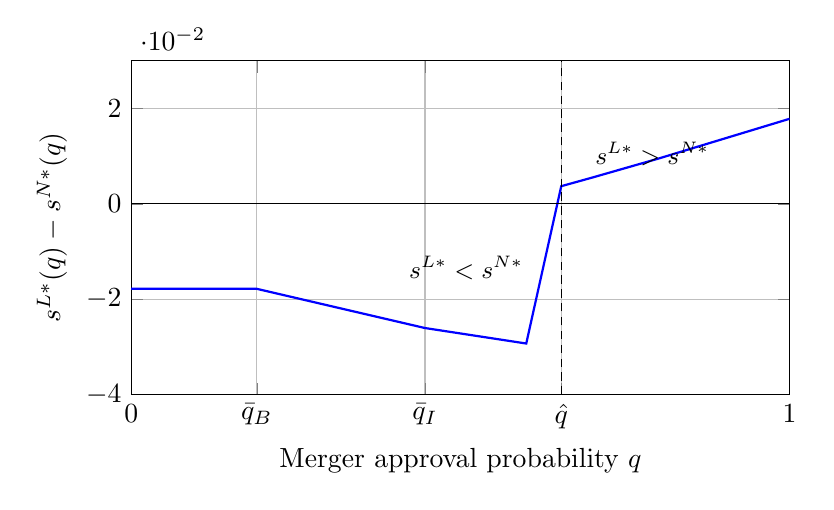
\begin{tikzpicture}
\begin{axis}[
    width=0.82\textwidth,
    height=0.48\textwidth,
    xmin=0, xmax=1,
    ymin=-0.04, ymax=0.03,
    xlabel={Merger approval probability \(q\)},
    ylabel={\(s^{L*}(q)-s^{N*}(q)\)},
    xtick={0,0.1907549041,0.4461335096,0.6531405543,1},
    xticklabels={0,\(\bar q_B\),\(\bar q_I\),\(\hat q\),1},
    ymajorgrids=true,
    xmajorgrids=true
]

\addplot[thick, blue] coordinates {
(0.00,-0.01784)
(0.1907549041,-0.01784)
(0.4461335096,-0.02606)
(0.60,-0.02931)
(0.6531405543,0.00369)
(0.70,0.00549)
(0.80,0.00945)
(1.00,0.01783)
};

\addplot[thin, black] coordinates {(0,0) (1,0)};
\addplot[densely dashed, black] coordinates {(0.6531405543,-0.04) (0.6531405543,0.03)};

\node[anchor=south east] at (axis cs:0.61,-0.018) {\small \(s^{L*}<s^{N*}\)};
\node[anchor=south west] at (axis cs:0.69,0.006) {\small \(s^{L*}>s^{N*}\)};
\end{axis}
\end{tikzpicture}
\caption{Transfer-augmented calibration illustrating sign reversal of the equilibrium subsidy wedge. The benchmark calibration from the main text is modified only by adding a locally retained buyout-proceeds term of size $0.70$ to approved local value for the buyout-oriented project.}
\label{fig:wedge_sign_reversal_appendix}
\end{figure}

\subsection{General distribution of entry costs}\label{app:nationalgeneralG}

Let entry costs be drawn from a continuously differentiable CDF \(G\) with density \(g\).
For project \(j\), the entry cutoff remains
\begin{equation}
    c_j(s,q)=s+\frac{R_j(q)^2}{2}.
\end{equation}
Aggregate national welfare is
\begin{equation}
    W_{j,G}^N(s,q)
    =
    \int_0^{c_j(s,q)}
    \left[
        R_j(q)B_j^N(q)
        -
        \frac{R_j(q)^2}{2}
        -
        f
        -
        \tau s
    \right] dG(f).
\end{equation}
Equivalently,
\begin{equation}
    W_{j,G}^N(s,q)
    =
    \left(
        R_j(q)B_j^N(q)
        -
        \frac{R_j(q)^2}{2}
        -
        \tau s
    \right)
    G(c_j)
    -
    \int_0^{c_j} f\,dG(f).
\end{equation}
Differentiating with respect to \(s\), using \(dc_j/ds=1\), yields the first-order condition
\begin{equation}
    g(c_j)
    \left[
        R_j(q)B_j^N(q)
        -
        R_j(q)^2
        -
        (\tau+1)s
    \right]
    -
    \tau G(c_j)
    =
    0.
\end{equation}
The uniform-distribution national formula in Section \ref{sec:decentralized} is the special case \(G(f)=f\).

\section{Appendix to Section \ref{sec:extensions}}\label{app:extensions}

\subsection{The merger-attempt condition under a clawback}

The clawback introduced in Section \ref{sec:extensions} is modeled as a reduced-form tax on the entrepreneur's merger-related continuation payoff.
It therefore changes the division of gains from acquisition, but not the joint surplus generated by attempting a merger.

Accordingly, the merger-attempt condition remains
\begin{equation}
    q\Delta_j \ge k.
\end{equation}
Equivalently, the attempt indicator is unchanged:
\begin{equation}
    a_j(q)=\mathbf{1}\{q\Delta_j \ge k\}.
\end{equation}
This distinction matters for welfare accounting.
Because the clawback does not affect product-market outcomes or merger feasibility, the local and national social-value objects \(B_j^L(q)\) and \(B_j^N(q)\) are unchanged.
Only private continuation values and therefore private effort, entry, and project choice are modified.
This assumption corresponds to a setting in which the clawback is imposed on the entrepreneur's realized continuation payoff after bargaining, rather than on the gross joint returns from merger attempt.
If the clawback also reduced the joint surplus from merger attempt, then the attempt threshold itself would shift; the present extension abstracts from that channel in order to isolate the composition effect of taxing entrepreneurial buyout returns.
For that reason, the extension should be read as a proof-of-concept policy-design exercise rather than as a full institutional model of clawback implementation.

\subsection{Project choice without the single-crossing restriction under a clawback}

Define the private payoff difference under a clawback:
\begin{equation}
    \widetilde D(q,\rho)\equiv \widetilde R_B(q,\rho)-\widetilde R_I(q,\rho).
\end{equation}
Using \eqref{eq:Rtilde}, this difference is
\begin{equation}\label{eq:Dqpiececlaw}
    \widetilde D(q,\rho)
    =
    \begin{cases}
        \pi_E^D(B)-\pi_E^D(I), &
        q < \bar q_B, \\
        \pi_E^D(B)-\pi_E^D(I)+(1-\rho)\beta(q\Delta_B-k), &
        \bar q_B \le q < \bar q_I, \\
        \pi_E^D(B)-\pi_E^D(I)+(1-\rho)\beta q(\Delta_B-\Delta_I), &
        q \ge \bar q_I,
    \end{cases}
\end{equation}
where
\begin{equation}
    \bar q_j\equiv \frac{k}{\Delta_j}.
\end{equation}

Because \(\pi_E^D(I)>\pi_E^D(B)\), we have
\begin{equation}
    \widetilde D(q,\rho)<0
    \qquad
    \text{for all } q<\bar q_B.
\end{equation}
In the intermediate region \([\bar q_B,\bar q_I)\), the buyout-oriented project is preferred if and only if
\begin{equation}\label{eq:qtilderho}
    q \ge \widetilde q(\rho)
    \equiv
    \frac{
        \pi_E^D(I)-\pi_E^D(B)+(1-\rho)\beta k
    }{
        (1-\rho)\beta\Delta_B
    }.
\end{equation}
Once both projects are merger-feasible, the buyout-oriented project is preferred if and only if
\begin{equation}\label{eq:qhatappendixrho}
    q \ge \hat q(\rho)
    \equiv
    \frac{
        \pi_E^D(I)-\pi_E^D(B)
    }{
        (1-\rho)\beta(\Delta_B-\Delta_I)
    }.
\end{equation}

Thus the clawback shifts upward both the intermediate-region threshold \(\widetilde q(\rho)\) and the full-feasibility threshold \(\hat q(\rho)\).
Under the maintained single-crossing structure used in the main text, attention can be restricted to the latter.

\subsection{Proof of Proposition \ref{prop:clawbackthreshold}}

Suppose both project types are merger-feasible, so that
\begin{equation}
    \widetilde R_j(q,\rho)
    =
    \pi_E^D(j)+(1-\rho)\beta(q\Delta_j-k),
    \qquad j\in\{I,B\}.
\end{equation}
The entrepreneur prefers project \(B\) if and only if
\begin{equation}
    \widetilde R_B(q,\rho)\ge \widetilde R_I(q,\rho).
\end{equation}
Substituting the expressions above yields
\begin{equation}
    \pi_E^D(B)+(1-\rho)\beta(q\Delta_B-k)
    \ge
    \pi_E^D(I)+(1-\rho)\beta(q\Delta_I-k).
\end{equation}
The \(-(1-\rho)\beta k\) terms cancel, so project \(B\) is preferred if and only if
\begin{equation}
    (1-\rho)\beta q(\Delta_B-\Delta_I)
    \ge
    \pi_E^D(I)-\pi_E^D(B).
\end{equation}
Since \(\Delta_B>\Delta_I\), this is equivalent to
\begin{equation}
    q\ge
    \hat q(\rho)
    \equiv
    \frac{
        \pi_E^D(I)-\pi_E^D(B)
    }{
        (1-\rho)\beta(\Delta_B-\Delta_I)
    }.
\end{equation}
This proves \eqref{eq:qhatrho}.

Differentiating \(\hat q(\rho)\) with respect to \(\rho\) gives
\begin{equation}
    \frac{\partial \hat q(\rho)}{\partial \rho}
    =
    \frac{
        \pi_E^D(I)-\pi_E^D(B)
    }{
        (1-\rho)^2\beta(\Delta_B-\Delta_I)
    }
    =
    \frac{\hat q(\rho)}{1-\rho}
    >0.
\end{equation}
This proves \eqref{eq:dqhatdrho}. \qed

\subsection{Derivation of the minimal clawback \eqref{eq:rhobar}}

Suppose \(q\) is such that both project types are merger-feasible.
To make project \(I\) privately optimal, it is sufficient to require
\begin{equation}
    q \le \hat q(\rho).
\end{equation}
Using \eqref{eq:qhatrho}, this becomes
\begin{equation}
    q
    \le
    \frac{
        \pi_E^D(I)-\pi_E^D(B)
    }{
        (1-\rho)\beta(\Delta_B-\Delta_I)
    }.
\end{equation}
Rearranging gives
\begin{equation}
    1-\rho
    \le
    \frac{
        \pi_E^D(I)-\pi_E^D(B)
    }{
        \beta q(\Delta_B-\Delta_I)
    }.
\end{equation}
Hence the smallest clawback that restores project \(I\) is
\begin{equation}
    \bar \rho(q)
    =
    1-
    \frac{
        \pi_E^D(I)-\pi_E^D(B)
    }{
        \beta q(\Delta_B-\Delta_I)
    }.
\end{equation}
Imposing the constraint \(\rho\ge 0\) yields \eqref{eq:rhobar}. \qed

\subsection{Modified welfare and subsidy formulas under a clawback}

Under the clawback extension, private continuation values are given by \(\widetilde R_j(q,\rho)\), and we define
\begin{equation}
    \widetilde A_j(q,\rho)\equiv \frac{\widetilde R_j(q,\rho)^2}{2},
    \qquad
    \widetilde c_j(s,q,\rho)\equiv s+\widetilde A_j(q,\rho).
\end{equation}
Because the clawback does not change realized product-market outcomes or the merger-attempt condition, the social-value objects \(B_j^L(q)\) and \(B_j^N(q)\) remain those defined in Sections \ref{sec:subsidy} and \ref{sec:decentralized}.

For the local planner,
\begin{equation}
    \widetilde W_j^L(s,q,\rho)
    =
    \widetilde c_j(s,q,\rho)
    \left(
        \widetilde R_j(q,\rho)B_j^L(q)
        -
        \widetilde A_j(q,\rho)
        -
        \tau s
    \right)
    -
    \frac{\widetilde c_j(s,q,\rho)^2}{2}.
\end{equation}
Expanding as in Appendix \ref{app:subsidy}, the derivative with respect to \(s\) is
\begin{equation}
    \frac{\partial \widetilde W_j^L(s,q,\rho)}{\partial s}
    =
    \widetilde R_j(q,\rho)B_j^L(q)
    -
    \frac{\tau+2}{2}\widetilde R_j(q,\rho)^2
    -
    (2\tau+1)s.
\end{equation}
Hence the local planner's type-specific optimal subsidy is
\begin{equation}
    \widetilde s_j^{L*}(q,\rho)
    =
    \max\left\{
        0,\;
        \frac{
            \widetilde R_j(q,\rho)B_j^L(q)
            -
            \frac{\tau+2}{2}\widetilde R_j(q,\rho)^2
        }{2\tau+1}
    \right\}.
\end{equation}

Similarly, the national planner's welfare under project \(j\) is
\begin{equation}
    \widetilde W_j^N(s,q,\rho)
    =
    \widetilde c_j(s,q,\rho)
    \left(
        \widetilde R_j(q,\rho)B_j^N(q)
        -
        \widetilde A_j(q,\rho)
        -
        \tau s
    \right)
    -
    \frac{\widetilde c_j(s,q,\rho)^2}{2},
\end{equation}
implying
\begin{equation}
    \widetilde s_j^{N*}(q,\rho)
    =
    \max\left\{
        0,\;
        \frac{
            \widetilde R_j(q,\rho)B_j^N(q)
            -
            \frac{\tau+2}{2}\widetilde R_j(q,\rho)^2
        }{2\tau+1}
    \right\}.
\end{equation}

Whenever both optimal subsidies are interior,
\begin{equation}
    \widetilde s_j^{L*}(q,\rho)-\widetilde s_j^{N*}(q,\rho)
    =
    \frac{
        \widetilde R_j(q,\rho)\bigl(B_j^L(q)-B_j^N(q)\bigr)
    }{2\tau+1}.
\end{equation}
Thus the clawback alters the magnitude of the local--national wedge through private continuation values, while holding fixed the underlying incidence difference between local and national welfare for a given project type.

\subsection{Proof of Proposition \ref{prop:instrumentsubstitution}}

The project-switching condition under a clawback is
\begin{equation}
    q(\theta)=\hat q(\rho).
\end{equation}
Differentiating totally with respect to \(\rho\) yields
\begin{equation}
    q'(\theta)\frac{d\theta}{d\rho}
    =
    \hat q'(\rho).
\end{equation}
Hence
\begin{equation}
    \frac{d\theta}{d\rho}
    =
    \frac{\hat q'(\rho)}{q'(\theta)}.
\end{equation}
Since \(q'(\theta)<0\) and Proposition \ref{prop:clawbackthreshold} implies \(\hat q'(\rho)>0\), it follows that
\begin{equation}
    \frac{d\theta}{d\rho}<0.
\end{equation}
Therefore a higher clawback rate permits a lower antitrust toughness while keeping the entrepreneur on the same project-indifference locus.

The second statement follows immediately from the condition for implementing project \(I\):
\begin{equation}
    q(\theta)\le \hat q(\rho).
\end{equation}
This inequality can be satisfied either by lowering \(q(\theta)\) through stricter antitrust, by raising \(\hat q(\rho)\) through a stronger clawback, or by adjusting both instruments jointly.
This proves the proposition. \qed


\section*{Funding}

This research did not receive any specific grant from funding agencies in the public, commercial, or not-for-profit sectors.

\section*{Declaration of competing interest}

The author declares that he has no known competing financial interests or personal relationships that could have appeared to influence the work reported in this paper.

\section*{Data availability}

No data were used for the research described in this article.

\section*{Declaration of generative AI and AI-assisted technologies in the writing process}

During the preparation of this work, the author used ChatGPT/Codex (OpenAI) in order to brainstorm and refine ideas and exposition, summarize and organize related literature, draft and edit portions of the manuscript for clarity and readability, and obtain suggestions for checking algebraic derivations and numerical verifications. After using this tool/service, the author reviewed and edited the content as needed and takes full responsibility for the content of the published article. The author independently verified all factual statements, citations, mathematical derivations, and computational results.

\bibliographystyle{plainnat}
\bibliography{refs}

\end{document}
